\subsection{Come le tipologie di messaggio verranno sfruttate}
Stabilito cos'è un Covert channel e lo scopo del protocollo ICMP; 
verrà indicato come le tipologie di messaggi presenti verranno sfruttate per esfiltrare dati fra due entità comunicanti.  

\subsubsection{Destination Unreachable Message (ICMPv4)} 
Nel protocollo \textbf{ICMPv4} la tipologia di messaggio \textit{Destination Unreachable}, 
viene usata quando la rete specificata (nel campo relativo alla destinazione di un datagram) è irraggiungibile. 
Di conseguenza il gateway potrà inviare questa tipologia di messaggio all'host mittente del pacchetto. 
\vspace{1ex} \newline 
Altri possibili caso potranno essere: l'host è irraggiungibile, 
il protocollo indicato o la porta di destinazione specificati non sono attivi, 
il pachcetto deve venrire frammetnato per poterlo inoltrare ad un gateway, 
\dots
\vspace{1ex} \newline 
Di seguito i codici associati ai possibili casi: 
\begin{itemize}
    \item \textcolor{red}{0} = net unreachable 
    \item \textcolor{red}{1} = host unreachable  
    \item \textcolor{blue}{2} = protocol unreachable  
    \item \textcolor{blue}{3} = port unreachable  
    \item \textcolor{red}{4} = fragmentation needed and DF set  
    \item \textcolor{red}{5} = source route failed 
\end{itemize}
I codici in rosso sono quelli ricevibili da un gateway mentre quelli blu potranno essere ricevuti da un host. 

\subsubsection*{Struttura del pacchetto} 
\begin{bytefield}[bitwidth=1.1em]{32} 
    %\bitbox{8}{0} & \bitbox{8}{1} & \bitbox{8}{2} & \bitbox{8}{3} \\
    \bitheader{0-31} \\
    \bitbox{8}{Type (1B)} & \bitbox{8}{Code (1B)} & \bitbox{16}{Checksum (2B)} \\
    \bitbox{32}{Unused (4B)} \\
    \bitbox{32}{Internet Header + 64 bits of Original Datagram ($\geq$ 21B)} 
\end{bytefield}
I campi sono i seguenti: 
\begin{itemize}
    \item Type: 3
    \item Code: 0-5 
    \item Checksum: è il complemento a 16 bit del complemento a uno relativo alla somma del messaggio ICMP 
    (che inizia con il campo Type). Verrà calcolato se il campo è zero.   
    \item  Internet Header + 64 bits of Data Datagram: 
    Questi dati vengono utilizzati dall'host per accoppiare il messaggio di errore al processo appropriato. 
    Se un protocollo di livello superiore utilizza numeri di porta, si presume che siano nei primi 64 bit dei dati del datagramma originale. 
    \footnote{L'\textit{intestazione IP} può variare dai 20 byte ai 40 byte} 
\end{itemize}
\vspace{1ex} 
Si sfrutteranno quindi i campi nel seguente modo: 
\begin{itemize}
    \item Il campo \textbf{checksum} non è utilizzabile. 
    Essendo il complemento ad 1 del contenuto del pacchetto, se non combaciasse il pacchetto verrebbe scartato. 
    \item Il campo \textbf{unused} dalle specifiche \href{https://www.rfc-editor.org/rfc/rfc792.html#:~:text=Destination%20Unreachable%20Message}{RFC 792} dovrebbe essere 0. 
    Tuttavia nel nostro caso è stato utilizzato per testare la presenza della \textit{Deep Packet Inspection}. 
    \item Nel campo \textbf{Header+64 bit} si userà il campo \textbf{len} del protocollo \textit{IP} e il campo \textbf{id} del protocollo \textit{ICMP}. 
    Tuttavia si dovrebbe inserire solo il primo byte del datagram originale. 
    Ciò cambierà la visibilità del pacchetto siccome non conforme allo standard. 
\end{itemize}

\subsubsection*{Analisi complessiva} 
Per l'analisi supponiamo di mandare due comandi che sono: 
\begin{itemize}
    \item \textbf{echo 'Ciao'}: che sono \textit{11 byte} (e quindi \textit{88 bit}\footnote{\label{note:destunreach:analisi}Ciò sarà utile per i \textit{Timing Covert Channel}})
    \item \textbf{cd /home/marco; ls -l}: che sono \textit{21 byte}  (e quindi \textit{168 bit}\textsuperscript{\ref{note:destunreach:analisi}}) %\footnotemark[2]
\end{itemize}
Sappiamo che nel caso migliore la capacità di trasmissione di ogni pacchetto è \textbf{8 byte} \label{destunreach:casoA}; 
mentre nel caso si vogliano rispettare le linee guida \href{https://www.rfc-editor.org/rfc/rfc792.html#:~:text=Destination%20Unreachable%20Message}{RFC 792}
non si potrà usare il campo \textit{unused} e si dovrà inserire solo il \textit{primo byte} del datagram originale. 
In questo secondo caso la capacità diventerà di \textbf{3 byte} \label{destunreach:casoB} siccome il campo \textit{len} verrà usato e in nel byte del datagram verrà messa un'informazione in più. 
Per ogni comando si confronteranno entrambe le varianti considerando che: 
\begin{itemize}
    \item Ogni pacchetto del primo caso (che chiameremo \hyperref[destunreach:casoA]{A}) trasporterà \textbf{36 byte} 
    \footnote{8 per i campi ICMP + 20 del datagram IP + 8 del datagram ICMP}
    \item Ogni pacchetto del secondo caso (che chiameremo \hyperref[destunreach:casoB]{B}) trasporterà \textbf{29 byte}
    \footnote{8 per i campi ICMP + 20 del datagram IP + 1 byte del datagram}
\end{itemize} 
Ora procediamo ad analizzare quanti pacchetti sono necessari per inviare i comandi. \newline
Nel caso si mandasse il comando \textbf{echo 'Ciao'} il numero di pacchetti necessari sarebbere: 
\begin{itemize}
    \item Caso \hyperref[destunreach:casoA]{A}: Sarebbero necessari \textit{due pacchetti}. 
    E quindi siccome ogni pacchetto trasporta 36 byte; si spediranno in totale \textbf{72 byte}.  
    \item Caso \hyperref[destunreach:casoB]{B}: Sarebbero necessari \textit{4 pacchetti}. 
     E quindi siccome ogni pacchetto trasporta 29 byte; si spediranno in totale \textbf{116 byte}. 
\end{itemize} 
Ora analiziamo il comando \textbf{cd /home/marco; ls -l} e quanti pacchetti saranno necessari: 
\begin{itemize}
    \item Caso \hyperref[destunreach:casoA]{A}: siccome è di \textit{21 byte}, servirebbero \textit{3 pacchetti}. 
    Quindi siccome ogni pacchetto trasporta 36 byte; si spediranno in totale \textbf{108 byte}.  
    \item Caso \hyperref[destunreach:casoB]{B}: siccome è di \textit{21 byte}, servirebbero \textit{7 pacchetti}. 
    Quindi siccome ogni pacchetto trasporta 29 byte; si spediranno in totale \textbf{203 byte}.  
\end{itemize}

\begin{center} 
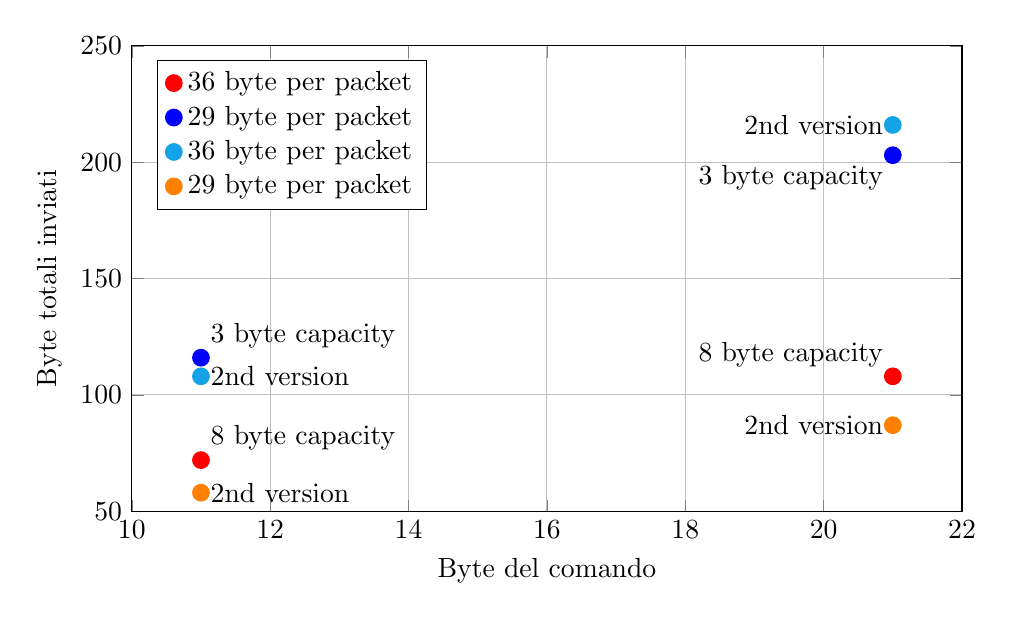
\begin{tikzpicture} 
    \tikzset{
    cmd11/.style={circle,fill=red,inner sep=2pt},
    cmd21/.style={circle,fill=blue,inner sep=2pt}
}
\begin{axis}[
    xlabel={Byte del comando}, 
    ylabel={Byte totali inviati},
    grid=major,
    width=\textwidth,
    height=0.618\textwidth, 
    domain=10:22,
    ymin=50,
    ymax=250, 
    legend pos=north west,
    legend entries={36 byte per packet, 29 byte per packet, 36 byte per packet, 29 byte per packet}
]  
% Plot points
\addplot[only marks, mark=*, mark size=3pt, red] 
coordinates {(11,72) (21,108)};
\addplot[only marks, mark=*, mark size=3pt, blue] 
coordinates {(11,116) (21,203)}; 
\addplot[only marks, mark=*, mark size=3pt, Cerulean] 
coordinates {(11,108) (21,216)}; 
\addplot[only marks, mark=*, mark size=3pt, orange] 
coordinates {(11,58) (21,87)}; 
% Add labels for the points 
\node[above right] at (axis cs:11,72) {8 byte capacity};
\node[above left] at (axis cs:21,108) {8 byte capacity};
\node[above right] at (axis cs:11,116) {3 byte capacity}; 
\node[below left] at (axis cs:21,203) {3 byte capacity}; 

\node[right] at (axis cs:11,108) {2nd version};
\node[left] at (axis cs:21,216) {2nd version};
\node[right] at (axis cs:11,58) {2nd version}; 
\node[left] at (axis cs:21,87) {2nd version}; 

\end{axis}
\end{tikzpicture}
\caption{Analisi tempi esecuzione \textit{Destination Unreachable}} 
\label{table:destunreach:bytetotali:bytecomando}
\end{center}
Dall'analisi segue che, per quanto errato nella costruzione, il metodo \hyperref[destunreach:casoA]{A} risulti il migliore. 
Infatti potrebbe essere facilmente rilevato semplicemente analizzando il campo \textit{unused} ma spedisce meno pacchetti per inviare il comando. 
Ciò risulta in un minor numero di bytes spediti in totale. 
\vspace{1ex} \newline 
Invece il secondo, per quanto corretto nelle norme, invia un numero considerevole di pacchetti (e quindi di bytes) rispetto alla controparte. 
Questo può rappresentare un problema maggiore perchè lo rende maggiormente rilevabile. 
Infatti un metodo di difesa potrebbe non accorgersi del campo \textit{unused} (qui usato correttamente) ma con molta probabilità si renderà conto della quantità di bytes inviati. 
\vspace{2ex} \newline
Una \textbf{soluzione} potrebbe essere quella di \textbf{usare il campo} \textit{unused} e 
\textbf{strutturare il pacchetto} nella seconda maniera; 
e quindi evitando tutta la parte ICMP del datagram. 
Ciò porta la \textit{capacità del pacchetto} a \textbf{7 byte} e i\textit{ byte per pacchetto} a \textbf{29 byte}. 
I risultati si possono vedere nel grafico [Tabel:\ref{table:destunreach:bytetotali:bytecomando} Arancione] 
\vspace{2ex} \newline
Invece una versione peggiore può essere fatta non inserendo i dati nel campo \textit{unused} ma mantendendo il datagram \textit{ICMP}. 
Ciò farà scendere la capacità del pacchetto a \textit{4 byte} mentre aumenterà i byte per pacchetto a \textit{36 byte}. 
I risultati si possono vedere nel grafico [Tabel:\ref{table:destunreach:bytetotali:bytecomando} Azzurro]. 

\subsubsection{Time Exceeded Message (ICMPv4)} 
Nel protocollo \textbf{ICMPv4} la tipologia di messaggio \textit{Time Exceeded}, 
viene usata quando il gateway che elabora un pacchetto trova che il suo TTL (tempo di vita) è zero. 
Di conseguenza il gateway dovrà scartare il datagramma e potrà poi notificare l'host sorgente della cosa tramite questa tipologia di messaggio. 
\vspace{1ex} \newline 
Altri possibili caso potranno essere: un host che riassembla un datagramma frammentato, non riesce a completare 
il riassemblaggio a causa di frammenti mancanti entro il proprio limite di tempo. 
\vspace{1ex} \newline 
Di seguito i codici associati ai possibili casi: 
\begin{itemize}
    \item \textcolor{red}{0} = TTL scaduto durante il transito 
    \item \textcolor{blue}{1} = tempo di riassemblaggio dei frammenti scaduto 
\end{itemize}
I codici in rosso sono quelli ricevibili da un gateway mentre quelli blu potranno essere ricevuti da un host.  

\subsubsection*{Struttura del pacchetto} 
\begin{bytefield}[bitwidth=1.1em]{32} 
    %\bitbox{8}{0} & \bitbox{8}{1} & \bitbox{8}{2} & \bitbox{8}{3} \\
    \bitheader{0-31} \\
    \bitbox{8}{Type (1B)} & \bitbox{8}{Code (1B)} & \bitbox{16}{Checksum (2B)} \\
    \bitbox{32}{Unused (4B)} \\
    \bitbox{32}{Internet Header + 64 bits of Original Datagram ($\geq$ 21B)} 
\end{bytefield}
I campi sono i seguenti: 
\begin{itemize}
    \item Type: 11
    \item Code: 0-1 
    \item Checksum: è il complemento a 16 bit del complemento a uno relativo alla somma del messaggio ICMP 
    (che inizia con il campo Type). Verrà calcolato se il campo è zero.   
    \item  Internet Header + 64 bits of Data Datagram: 
    Questi dati vengono utilizzati dall'host per accoppiare il messaggio di errore al processo appropriato. 
    Se un protocollo di livello superiore utilizza numeri di porta, si presume che siano nei primi 64 bit dei dati del datagramma originale. 
    \footnote{L'\textit{intestazione IP} può variare dai 20 byte ai 40 byte} 
\end{itemize}
\vspace{1ex} 
Si sfrutteranno quindi i campi nel seguente modo: 
\begin{itemize}
    \item Il campo \textbf{checksum} non è utilizzabile. 
    Essendo il complemento ad 1 del contenuto del pacchetto, se non combaciasse il pacchetto verrebbe scartato. 
    \item Il campo \textbf{unused} dalle specifiche \href{https://www.rfc-editor.org/rfc/rfc792.html#:~:text=Time%20Exceeded%20Message}{RFC 792} dovrebbe essere 0. 
    Tuttavia nel nostro caso è stato utilizzato per testare la presenza della \textit{Deep Packet Inspection}. 
    \item Nel campo \textbf{Header+64 bit} si userà il campo \textbf{len} del protocollo \textit{IP} e il campo \textbf{id} del protocollo \textit{ICMP}. 
    Tuttavia si dovrebbe inserire solo il primo byte del datagram originale. 
    Ciò cambierà la visibilità del pacchetto siccome non conforme allo standard. 
\end{itemize}

\subsubsection*{Analisi complessiva} 
Per l'analisi supponiamo di mandare due comandi che sono: 
\begin{itemize}
    \item \textbf{echo 'Ciao'}: che sono \textit{11 byte} (e quindi \textit{88 bit}\footnote{\label{note:timeexceed:analisi}Ciò sarà utile per i \textit{Timing Covert Channel}})
    \item \textbf{cd /home/marco; ls -l}: che sono \textit{21 byte}  (e quindi \textit{168 bit}\textsuperscript{\ref{note:timeexceed:analisi}}) %\footnotemark[2]
\end{itemize}
Sappiamo che nel caso migliore la capacità di trasmissione di ogni pacchetto è \textbf{8 byte} \label{timeexceed:casoA}; 
mentre nel caso si vogliano rispettare le linee guida \href{https://www.rfc-editor.org/rfc/rfc792.html#:~:text=Time%20Exceeded%20Message}{RFC 792}
non si potrà usare il campo \textit{unused} e si dovrà inserire solo il \textit{primo byte} del datagram originale. 
In questo secondo caso la capacità diventerà di \textbf{3 byte} \label{timeexceed:casoB} siccome il campo \textit{len} verrà usato e in nel byte del datagram verrà messa un'informazione in più. 
Per ogni comando si confronteranno entrambe le varianti considerando che: 
\begin{itemize}
    \item Ogni pacchetto del primo caso (che chiameremo \hyperref[timeexceed:casoA]{A}) trasporterà \textbf{36 byte} 
    \footnote{8 per i campi ICMP + 20 del datagram IP + 8 del datagram ICMP}
    \item Ogni pacchetto del secondo caso (che chiameremo \hyperref[timeexceed:casoB]{B}) trasporterà \textbf{29 byte}
    \footnote{8 per i campi ICMP + 20 del datagram IP + 1 byte del datagram}
\end{itemize} 
Ora procediamo ad analizzare quanti pacchetti sono necessari per inviare i comandi. \newline
Nel caso si mandasse il comando \textbf{echo 'Ciao'} il numero di pacchetti necessari sarebbere: 
\begin{itemize}
    \item Caso \hyperref[timeexceed:casoA]{A}: Sarebbero necessari \textit{due pacchetti}. 
    E quindi siccome ogni pacchetto trasporta 36 byte; si spediranno in totale \textbf{72 byte}.  
    \item Caso \hyperref[timeexceed:casoB]{B}: Sarebbero necessari \textit{4 pacchetti}. 
     E quindi siccome ogni pacchetto trasporta 29 byte; si spediranno in totale \textbf{116 byte}. 
\end{itemize} 
Ora analiziamo il comando \textbf{cd /home/marco; ls -l} e quanti pacchetti saranno necessari: 
\begin{itemize}
    \item Caso \hyperref[timeexceed:casoA]{A}: siccome è di \textit{21 byte}, servirebbero \textit{3 pacchetti}. 
    Quindi siccome ogni pacchetto trasporta 36 byte; si spediranno in totale \textbf{108 byte}.  
    \item Caso \hyperref[timeexceed:casoB]{B}: siccome è di \textit{21 byte}, servirebbero \textit{7 pacchetti}. 
    Quindi siccome ogni pacchetto trasporta 29 byte; si spediranno in totale \textbf{203 byte}.  
\end{itemize}

\begin{center} 
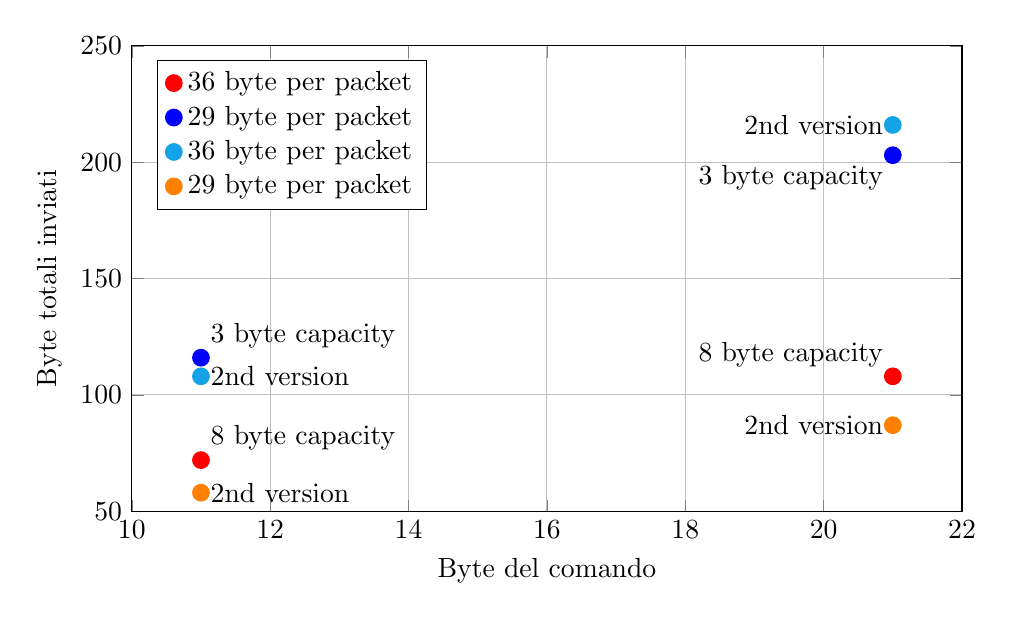
\begin{tikzpicture} 
    \tikzset{
    cmd11/.style={circle,fill=red,inner sep=2pt},
    cmd21/.style={circle,fill=blue,inner sep=2pt}
}
\begin{axis}[
    xlabel={Byte del comando}, 
    ylabel={Byte totali inviati},
    grid=major,
    width=\textwidth,
    height=0.618\textwidth, 
    domain=10:22,
    ymin=50,
    ymax=250, 
    legend pos=north west,
    legend entries={36 byte per packet, 29 byte per packet, 36 byte per packet, 29 byte per packet}
]  
% Plot points
\addplot[only marks, mark=*, mark size=3pt, red] 
coordinates {(11,72) (21,108)};
\addplot[only marks, mark=*, mark size=3pt, blue] 
coordinates {(11,116) (21,203)}; 
\addplot[only marks, mark=*, mark size=3pt, Cerulean] 
coordinates {(11,108) (21,216)}; 
\addplot[only marks, mark=*, mark size=3pt, orange] 
coordinates {(11,58) (21,87)}; 
% Add labels for the points 
\node[above right] at (axis cs:11,72) {8 byte capacity};
\node[above left] at (axis cs:21,108) {8 byte capacity};
\node[above right] at (axis cs:11,116) {3 byte capacity}; 
\node[below left] at (axis cs:21,203) {3 byte capacity}; 

\node[right] at (axis cs:11,108) {2nd version};
\node[left] at (axis cs:21,216) {2nd version};
\node[right] at (axis cs:11,58) {2nd version}; 
\node[left] at (axis cs:21,87) {2nd version}; 

\end{axis}
\end{tikzpicture}
\caption{Analisi tempi esecuzione \textit{Time Excedeed}} 
\label{table:timeexceed:bytetotali:bytecomando}
\end{center}
Dall'analisi segue che, per quanto errato nella costruzione, il metodo \hyperref[timeexceed:casoA]{A} risulti il migliore. 
Infatti potrebbe essere facilmente rilevato semplicemente analizzando il campo \textit{unused} ma spedisce meno pacchetti per inviare il comando. 
Ciò risulta in un minor numero di bytes spediti in totale. 
\vspace{1ex} \newline 
Invece il secondo, per quanto corretto nelle norme, invia un numero considerevole di pacchetti (e quindi di bytes) rispetto alla controparte. 
Questo può rappresentare un problema maggiore perchè lo rende maggiormente rilevabile. 
Infatti un metodo di difesa potrebbe non accorgersi del campo \textit{unused} (qui usato correttamente) ma con molta probabilità si renderà conto della quantità di bytes inviati. 
\vspace{2ex} \newline
Una \textbf{soluzione} potrebbe essere quella di \textbf{usare il campo} \textit{unused} e 
\textbf{strutturare il pacchetto} nella seconda maniera; 
e quindi evitando tutta la parte ICMP del datagram. 
Ciò porta la \textit{capacità del pacchetto} a \textbf{7 byte} e i\textit{ byte per pacchetto} a \textbf{29 byte}. 
I risultati si possono vedere nel grafico [Tabel:\ref{table:timeexceed:bytetotali:bytecomando} Arancione] 
\vspace{2ex} \newline
Invece una versione peggiore può essere fatta non inserendo i dati nel campo \textit{unused} ma mantendendo il datagram \textit{ICMP}. 
Ciò farà scendere la capacità del pacchetto a \textit{4 byte} mentre aumenterà i byte per pacchetto a \textit{36 byte}. 
I risultati si possono vedere nel grafico [Tabel:\ref{table:timeexceed:bytetotali:bytecomando} Azzurro]. 

\subsubsection{Parameter Problem Message (ICMPv4)} 
Nel protocollo \textbf{ICMPv4} la tipologia di messaggio \textit{Parameter Problem}, 
viene usata quando il gateway che elabora un pacchetto  trova un problema con i parametri dell'intestazione in modo tale da non poter completare l'elaborazione del datagramma. 
In questo caso dovrà scartare il datagramma e potrà notificare l'host sorgente della cosa tramite questa tipologia di messaggio. 
\vspace{1ex} \newline 
Una potenziale sorgente di tale problema è rappresentata da argomenti non corretti in un'opzione. 
E questo messaggio viene inviato solo se l'errore ha causato lo scarto del pacchetto. 
\vspace{1ex} \newline 
Di seguito i codici associati ai possibili casi: 
\begin{itemize}
    \item \textcolor{red}{0} = TTL scaduto durante il transito 
    \item \textcolor{blue}{1} = tempo di riassemblaggio dei frammenti scaduto 
\end{itemize}
I codici in rosso sono quelli ricevibili da un gateway mentre quelli blu potranno essere ricevuti da un host.  

\subsubsection*{Struttura del pacchetto} 
\begin{bytefield}[bitwidth=1.1em]{32} 
    %\bitbox{8}{0} & \bitbox{8}{1} & \bitbox{8}{2} & \bitbox{8}{3} \\
    \bitheader{0-31} \\
    \bitbox{8}{Type (1B)} & \bitbox{8}{Code (1B)} & \bitbox{16}{Checksum (2B)} \\
    \bitbox{8}{Pointer (1B)} & \bitbox{24}{Unused (3B)} \\
    \bitbox{32}{Internet Header + 64 bits of Original Datagram ($\geq$ 21B)} 
\end{bytefield}
I campi sono i seguenti: 
\begin{itemize}
    \item Type: 12
    \item Code: 0 e il puntatore indicherà l'errore
    \item Checksum: è il complemento a 16 bit del complemento a uno relativo alla somma del messaggio ICMP 
    (che inizia con il campo Type). Verrà calcolato se il campo è zero.  
    \item Puntatore: se il codice è 0, identifica l'ottetto in cui è stato rilevato un errore. 
    \item Internet Header + 64 bits of Data Datagram: 
    Questi dati vengono utilizzati dall'host per accoppiare il messaggio di errore al processo appropriato. 
    Se un protocollo di livello superiore utilizza numeri di porta, si presume che siano nei primi 64 bit dei dati del datagramma originale. 
    \footnote{L'\textit{intestazione IP} può variare dai 20 byte ai 40 byte} 
\end{itemize}
Il puntatore identifica l'ottetto dell'intestazione originale del datagramma in cui è 
stato rilevato l'errore (può trovarsi nel mezzo di un'opzione). 
Ad esempio, 1 indica che c'è qualcosa di sbagliato con il Tipo di Servizio, e (se sono presenti opzioni) 20 indica che 
c'è qualcosa di sbagliato con il codice di tipo della prima opzione. 
Il codice 0 può essere ricevuto da un gateway o da un host.
\vspace{1ex} 
Si sfrutteranno quindi i campi nel seguente modo: 
\begin{itemize}
    \item Il campo \textbf{checksum} non è utilizzabile. 
    Essendo il complemento ad 1 del contenuto del pacchetto, se non combaciasse il pacchetto verrebbe scartato. 
    \item Il campo \textbf{pointer} dovrebbe rappresentare l'ottetto in cui è avvenuto l'errore. 
    Tuttavia potrebbe contenere dei dati non correlati ad esso. 
    \item Il campo \textbf{unused} dalle specifiche \href{https://www.rfc-editor.org/rfc/rfc792.html#:~:text=Parameter%%20Problem%%20Message}{RFC 792} dovrebbe essere 0. 
    Tuttavia nel nostro caso è stato utilizzato per testare la presenza della \textit{Deep Packet Inspection}. 
    \item Nel campo \textbf{Header+64 bit} si userà il campo \textbf{len} del protocollo \textit{IP} e il campo \textbf{id} del protocollo \textit{ICMP}. 
    Tuttavia si dovrebbe inserire solo il primo byte del datagram originale. 
    Ciò cambierà la visibilità del pacchetto siccome non conforme allo standard. 
\end{itemize}

\subsubsection*{Analisi complessiva} 
Per l'analisi supponiamo di mandare due comandi che sono: 
\begin{itemize}
    \item \textbf{echo 'Ciao'}: che sono \textit{11 byte} (e quindi \textit{88 bit}\footnote{\label{note:paramprobl:analisi}Ciò sarà utile per i \textit{Timing Covert Channel}})
    \item \textbf{cd /home/marco; ls -l}: che sono \textit{21 byte}  (e quindi \textit{168 bit}\textsuperscript{\ref{note:paramprobl:analisi}}) %\footnotemark[2]
\end{itemize}
Sappiamo che nel caso migliore la capacità di trasmissione di ogni pacchetto è \textbf{8 byte} \label{paramprobl:casoA}; %%20
mentre nel caso si vogliano rispettare le linee guida \href{https://www.rfc-editor.org/rfc/rfc792.html#:~:text=Parameter%%20Problem%%20Message}{RFC 792}
non si potrà usare il campo \textit{unused} e si dovrà inserire solo il \textit{primo byte} del datagram originale. 
In questo secondo caso la capacità diventerà di \textbf{4 byte} \label{paramprobl:casoB} siccome il campo \textit{pntr} e \textit{len} verranno usati e in nel byte del datagram verrà messa un'informazione in più. 
Per ogni comando si confronteranno entrambe le varianti considerando che: 
\begin{itemize}
    \item Ogni pacchetto del primo caso (che chiameremo \hyperref[paramprobl:casoA]{A}) trasporterà \textbf{36 byte} 
    \footnote{8 per i campi ICMP + 20 del datagram IP + 8 del datagram ICMP}
    \item Ogni pacchetto del secondo caso (che chiameremo \hyperref[paramprobl:casoB]{B}) trasporterà \textbf{29 byte}
    \footnote{8 per i campi ICMP + 20 del datagram IP + 1 byte del datagram}
\end{itemize} 
Ora procediamo ad analizzare quanti pacchetti sono necessari per inviare i comandi. \newline
Nel caso si mandasse il comando \textbf{echo 'Ciao'} il numero di pacchetti necessari sarebbere: 
\begin{itemize}
    \item Caso \hyperref[paramprobl:casoA]{A}: Sarebbero necessari \textit{due pacchetti}. 
    E quindi siccome ogni pacchetto trasporta 36 byte; si spediranno in totale \textbf{72 byte}.  
    \item Caso \hyperref[paramprobl:casoB]{B}: Sarebbero necessari \textit{3 pacchetti}. 
     E quindi siccome ogni pacchetto trasporta 29 byte; si spediranno in totale \textbf{87 byte}. 
\end{itemize} 
Ora analiziamo il comando \textbf{cd /home/marco; ls -l} e quanti pacchetti saranno necessari: 
\begin{itemize}
    \item Caso \hyperref[paramprobl:casoA]{A}: siccome è di \textit{21 byte}, servirebbero \textit{3 pacchetti}. 
    Quindi siccome ogni pacchetto trasporta 36 byte; si spediranno in totale \textbf{108 byte}.  
    \item Caso \hyperref[paramprobl:casoB]{B}: siccome è di \textit{21 byte}, servirebbero \textit{7 pacchetti}. 
    Quindi siccome ogni pacchetto trasporta 29 byte; si spediranno in totale \textbf{174 byte}. 
\end{itemize}

\begin{center} 
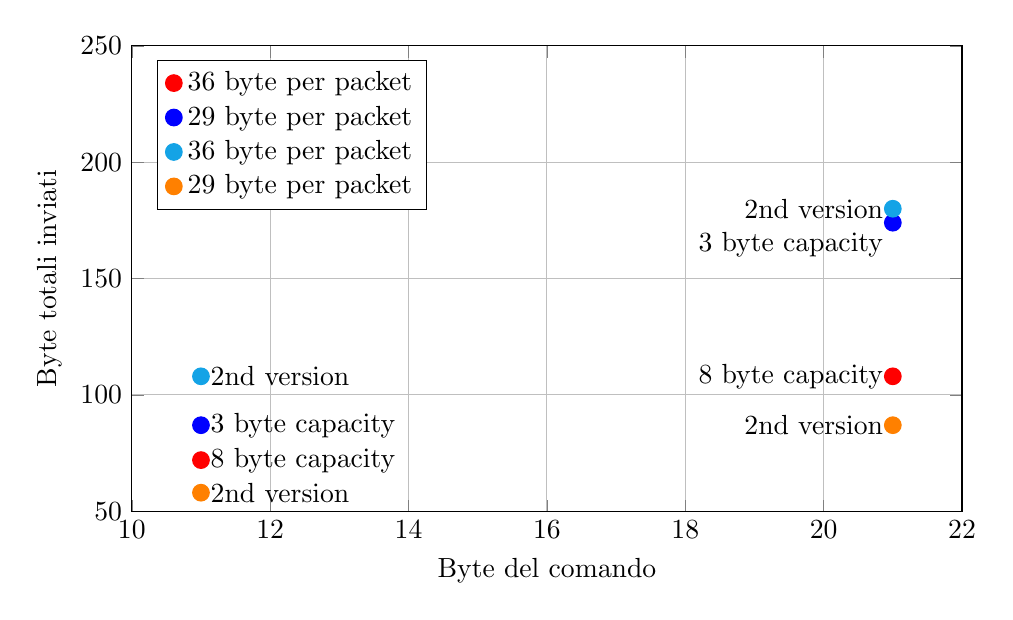
\begin{tikzpicture} 
    \tikzset{
    cmd11/.style={circle,fill=red,inner sep=2pt},
    cmd21/.style={circle,fill=blue,inner sep=2pt}
}
\begin{axis}[
    xlabel={Byte del comando}, 
    ylabel={Byte totali inviati},
    grid=major,
    width=\textwidth,
    height=0.618\textwidth, 
    domain=10:22,
    ymin=50,
    ymax=250, 
    legend pos=north west,
    legend entries={36 byte per packet, 29 byte per packet, 36 byte per packet, 29 byte per packet}
]  
% Plot points
\addplot[only marks, mark=*, mark size=3pt, red] 
coordinates {(11,72) (21,108)};
\addplot[only marks, mark=*, mark size=3pt, blue] 
coordinates {(11,87) (21,174)}; 
\addplot[only marks, mark=*, mark size=3pt, Cerulean] 
coordinates {(11,108) (21,180)}; 
\addplot[only marks, mark=*, mark size=3pt, orange] 
coordinates {(11,58) (21,87)}; 
% Add labels for the points 
\node[right] at (axis cs:11,72) {8 byte capacity};
\node[left] at (axis cs:21,108) {8 byte capacity};
\node[right] at (axis cs:11,87) {3 byte capacity}; 
\node[below left] at (axis cs:21,174) {3 byte capacity}; 

\node[right] at (axis cs:11,108) {2nd version};
\node[left] at (axis cs:21,180) {2nd version};
\node[right] at (axis cs:11,58) {2nd version}; 
\node[left] at (axis cs:21,87) {2nd version}; 

\end{axis}
\end{tikzpicture}
\caption{Analisi tempi esecuzione \textit{Parameter Problem}} 
\label{table:paramprobl:bytetotali:bytecomando}
\end{center}
Dall'analisi segue che, per quanto errato nella costruzione, il metodo \hyperref[paramprobl:casoA]{A} risulti il migliore. 
Infatti potrebbe essere facilmente rilevato semplicemente analizzando il campo \textit{unused} ma spedisce meno pacchetti per inviare il comando. 
Ciò risulta in un minor numero di bytes spediti in totale. 
\vspace{1ex} \newline 
Invece il secondo, per quanto corretto nelle norme, invia un numero considerevole di pacchetti (e quindi di bytes) rispetto alla controparte. 
Questo può rappresentare un problema maggiore perchè lo rende maggiormente rilevabile. 
Infatti un metodo di difesa potrebbe non accorgersi del campo \textit{unused} (qui usato correttamente) ma con molta probabilità si renderà conto della quantità di bytes inviati. 
\vspace{2ex} \newline
Una \textbf{soluzione} potrebbe essere quella di \textbf{usare il campo} \textit{unused} e 
\textbf{strutturare il pacchetto} nella seconda maniera; 
e quindi evitando tutta la parte ICMP del datagram. 
Ciò porta la \textit{capacità del pacchetto} a \textbf{7 byte} e i\textit{ byte per pacchetto} a \textbf{29 byte}. 
I risultati si possono vedere nel grafico [Tabel:\ref{table:paramprobl:bytetotali:bytecomando} Arancione] 
\vspace{2ex} \newline
Invece una versione peggiore può essere fatta non inserendo i dati nel campo \textit{unused} ma mantendendo il datagram \textit{ICMP}. 
Ciò farà scendere la capacità del pacchetto a \textit{5 byte} mentre aumenterà i byte per pacchetto a \textit{36 byte}. 
I risultati si possono vedere nel grafico [Tabel:\ref{table:paramprobl:bytetotali:bytecomando} Azzurro]. 

\subsubsection{Source Quench Message (ICMPv4)} 
Nel protocollo \textbf{ICMPv4} la tipologia di messaggio \textit{Source Quench}, viene usata quando il gateway gateway scarta un pacchetto;  
in questo caso potrà inviare un messaggio di Source Quench all'host Internet mittente. 
Un gateway può scartare un pacchetto se non ha lo spazio necessario nel buffer 
per mantenere in coda i pacchetti che dovranno essere inoltrati alla rete successiva; 
la quale dovrà far parte della rotta per la rete di destinazione. 
%per l'uscita verso la rete successiva nella rotta per la rete di destinazione. 
Il gateway può inviare un messaggio di attenuazione della sorgente per ogni messaggio che scarta. 
\vspace{1ex} \newline 
Un host di destinazione può inviare un messaggio di Source Quench anche nel caso in cui i datagrammi arrivino troppo velocemente per essere elaborati.
Ciò indicherà una richiesta da parte dell'host destinatario all'host mittente, di ridurre la velocità con cui si stanno inviando i pacchetti nel traffico. 
Al suo ricevimento, l'host sorgente dovrà ridurre la velocità sino a quando non riceverà più messaggi Source Quench dal gateway.
L'host mittente potrà successivamente aumentare gradualmente la velocità con cui sta inviando i pacchetti fino a quando non riceverà nuovamente questi messaggi.
\vspace{1ex} \newline 
Il gateway o l'host può inoltre inviare il messaggio di Source Quench anche quando si avvicina al limite di capacità; 
piuttosto che aspettare e lasciare che questa capacità venga superata. 
Questo porterà al vantaggio che il pacchetto che ha attivato il messaggio potrebbe essere consegnato; 
mentre nel caso precedente non vi era abbastanza spazio per poterlo memorizzare (siccome la coda è piena). 
%\vspace{1ex} \newline 
%Di seguito i codici associati ai possibili casi: 
%\begin{itemize}
%    \item \textcolor{red}{0} = TTL scaduto durante il transito 
%    \item \textcolor{blue}{1} = tempo di riassemblaggio dei frammenti scaduto 
%\end{itemize}
%I codici in rosso sono quelli ricevibili da un gateway mentre quelli blu potranno essere ricevuti da un host.  

\subsubsection*{Struttura del pacchetto} 
\begin{bytefield}[bitwidth=1.1em]{32} 
    %\bitbox{8}{0} & \bitbox{8}{1} & \bitbox{8}{2} & \bitbox{8}{3} \\
    \bitheader{0-31} \\
    \bitbox{8}{Type (1B)} & \bitbox{8}{Code (1B)} & \bitbox{16}{Checksum (2B)} \\
    \bitbox{32}{Unused (4B)} \\
    \bitbox{32}{Internet Header + 64 bits of Original Datagram ($\geq$ 21B)} 
\end{bytefield}
I campi sono i seguenti: 
\begin{itemize}
    \item Type: 4 
    \item Code: 0 il codice 0 può essere ricevuto da un gateway o un host 
    \item Checksum: è il complemento a 16 bit del complemento a uno relativo alla somma del messaggio ICMP 
    (che inizia con il campo Type). Verrà calcolato se il campo è zero.   
    \item  Internet Header + 64 bits of Data Datagram: 
    Questi dati vengono utilizzati dall'host per accoppiare il messaggio di errore al processo appropriato. 
    Se un protocollo di livello superiore utilizza numeri di porta, si presume che siano nei primi 64 bit dei dati del datagramma originale. 
    \footnote{L'\textit{intestazione IP} può variare dai 20 byte ai 40 byte} 
\end{itemize}
\vspace{1ex} 
Si sfrutteranno quindi i campi nel seguente modo: 
\begin{itemize}
    \item Il campo \textbf{checksum} non è utilizzabile. 
    Essendo il complemento ad 1 del contenuto del pacchetto, se non combaciasse il pacchetto verrebbe scartato. 
    \item Il campo \textbf{unused} dalle specifiche \href{https://www.rfc-editor.org/rfc/rfc792.html#:~:text=Source%20Quench%20Message}{RFC 792} dovrebbe essere 0. 
    Tuttavia nel nostro caso è stato utilizzato per testare la presenza della \textit{Deep Packet Inspection}. 
    \item Nel campo \textbf{Header+64 bit} si userà il campo \textbf{len} del protocollo \textit{IP} e il campo \textbf{id} del protocollo \textit{ICMP}. 
    Tuttavia si dovrebbe inserire solo il primo byte del datagram originale. 
    Ciò cambierà la visibilità del pacchetto siccome non conforme allo standard. 
\end{itemize}

\subsubsection*{Analisi complessiva} 
Per l'analisi supponiamo di mandare due comandi che sono: 
\begin{itemize}
    \item \textbf{echo 'Ciao'}: che sono \textit{11 byte} (e quindi \textit{88 bit}\footnote{\label{note:srcquench:analisi}Ciò sarà utile per i \textit{Timing Covert Channel}})
    \item \textbf{cd /home/marco; ls -l}: che sono \textit{21 byte}  (e quindi \textit{168 bit}\textsuperscript{\ref{note:srcquench:analisi}}) %\footnotemark[2]
\end{itemize}
Sappiamo che nel caso migliore la capacità di trasmissione di ogni pacchetto è \textbf{8 byte} \label{srcquench:casoA}; %20
mentre nel caso si vogliano rispettare le linee guida \href{https://www.rfc-editor.org/rfc/rfc792.html#:~:text=Source%20Quench%20Message}{RFC 792}
non si potrà usare il campo \textit{unused} e si dovrà inserire solo il \textit{primo byte} del datagram originale. 
In questo secondo caso la capacità diventerà di \textbf{3 byte} \label{srcquench:casoB} siccome il campo \textit{len} verrà usato e in nel byte del datagram verrà messa un'informazione in più. 
Per ogni comando si confronteranno entrambe le varianti considerando che: 
\begin{itemize}
    \item Ogni pacchetto del primo caso (che chiameremo \hyperref[srcquench:casoA]{A}) trasporterà \textbf{36 byte} 
    \footnote{8 per i campi ICMP + 20 del datagram IP + 8 del datagram ICMP}
    \item Ogni pacchetto del secondo caso (che chiameremo \hyperref[srcquench:casoB]{B}) trasporterà \textbf{29 byte}
    \footnote{8 per i campi ICMP + 20 del datagram IP + 1 byte del datagram}
\end{itemize} 
Ora procediamo ad analizzare quanti pacchetti sono necessari per inviare i comandi. \newline
Nel caso si mandasse il comando \textbf{echo 'Ciao'} il numero di pacchetti necessari sarebbere: 
\begin{itemize}
    \item Caso \hyperref[srcquench:casoA]{A}: Sarebbero necessari \textit{due pacchetti}. 
    E quindi siccome ogni pacchetto trasporta 36 byte; si spediranno in totale \textbf{72 byte}.  
    \item Caso \hyperref[srcquench:casoB]{B}: Sarebbero necessari \textit{4 pacchetti}. 
     E quindi siccome ogni pacchetto trasporta 29 byte; si spediranno in totale \textbf{116 byte}. 
\end{itemize} 
Ora analiziamo il comando \textbf{cd /home/marco; ls -l} e quanti pacchetti saranno necessari: 
\begin{itemize}
    \item Caso \hyperref[srcquench:casoA]{A}: siccome è di \textit{21 byte}, servirebbero \textit{3 pacchetti}. 
    Quindi siccome ogni pacchetto trasporta 36 byte; si spediranno in totale \textbf{108 byte}.  
    \item Caso \hyperref[srcquench:casoB]{B}: siccome è di \textit{21 byte}, servirebbero \textit{7 pacchetti}. 
    Quindi siccome ogni pacchetto trasporta 29 byte; si spediranno in totale \textbf{203 byte}.  
\end{itemize}

\begin{center} 
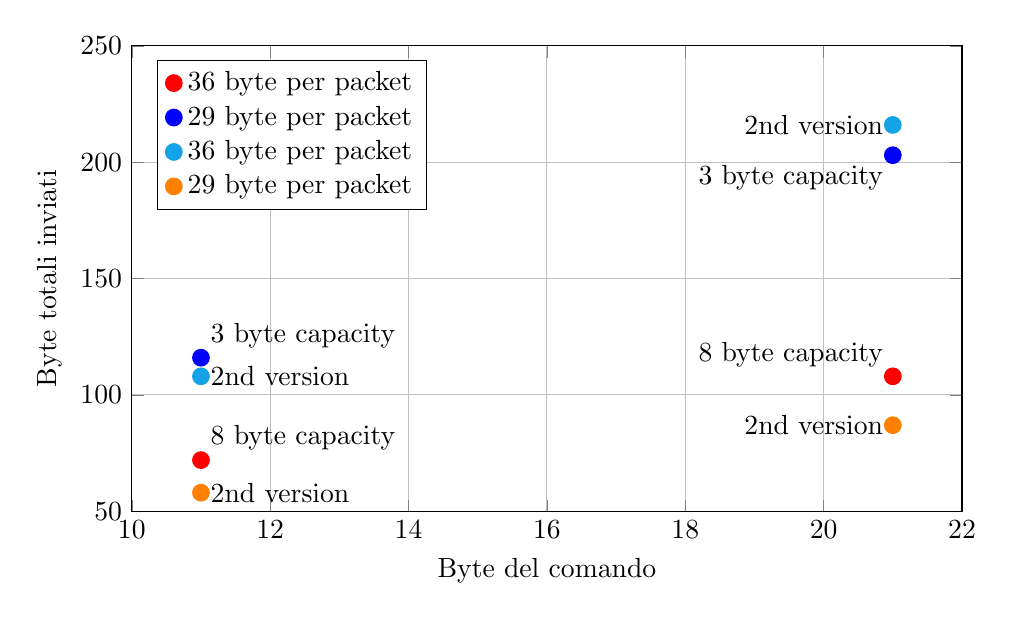
\begin{tikzpicture} 
    \tikzset{
    cmd11/.style={circle,fill=red,inner sep=2pt},
    cmd21/.style={circle,fill=blue,inner sep=2pt}
}
\begin{axis}[
    xlabel={Byte del comando}, 
    ylabel={Byte totali inviati},
    grid=major,
    width=\textwidth,
    height=0.618\textwidth, 
    domain=10:22,
    ymin=50,
    ymax=250, 
    legend pos=north west,
    legend entries={36 byte per packet, 29 byte per packet, 36 byte per packet, 29 byte per packet}
]  
% Plot points
\addplot[only marks, mark=*, mark size=3pt, red] 
coordinates {(11,72) (21,108)};
\addplot[only marks, mark=*, mark size=3pt, blue] 
coordinates {(11,116) (21,203)}; 
\addplot[only marks, mark=*, mark size=3pt, Cerulean] 
coordinates {(11,108) (21,216)}; 
\addplot[only marks, mark=*, mark size=3pt, orange] 
coordinates {(11,58) (21,87)}; 
% Add labels for the points 
\node[above right] at (axis cs:11,72) {8 byte capacity};
\node[above left] at (axis cs:21,108) {8 byte capacity};
\node[above right] at (axis cs:11,116) {3 byte capacity}; 
\node[below left] at (axis cs:21,203) {3 byte capacity}; 

\node[right] at (axis cs:11,108) {2nd version};
\node[left] at (axis cs:21,216) {2nd version};
\node[right] at (axis cs:11,58) {2nd version}; 
\node[left] at (axis cs:21,87) {2nd version}; 

\end{axis}
\end{tikzpicture}
\caption{Analisi tempi esecuzione \textit{Source Quench}} 
\label{table:srcquench:bytetotali:bytecomando}
\end{center}
Dall'analisi segue che, per quanto errato nella costruzione, il metodo \hyperref[srcquench:casoA]{A} risulti il migliore. 
Infatti potrebbe essere facilmente rilevato semplicemente analizzando il campo \textit{unused} ma spedisce meno pacchetti per inviare il comando. 
Ciò risulta in un minor numero di bytes spediti in totale. 
\vspace{1ex} \newline 
Invece il secondo, per quanto corretto nelle norme, invia un numero considerevole di pacchetti (e quindi di bytes) rispetto alla controparte. 
Questo può rappresentare un problema maggiore perchè lo rende maggiormente rilevabile. 
Infatti un metodo di difesa potrebbe non accorgersi del campo \textit{unused} (qui usato correttamente) ma con molta probabilità si renderà conto della quantità di bytes inviati. 
\vspace{2ex} \newline
Una \textbf{soluzione} potrebbe essere quella di \textbf{usare il campo} \textit{unused} e 
\textbf{strutturare il pacchetto} nella seconda maniera; 
e quindi evitando tutta la parte ICMP del datagram. 
Ciò porta la \textit{capacità del pacchetto} a \textbf{7 byte} e i\textit{ byte per pacchetto} a \textbf{29 byte}. 
I risultati si possono vedere nel grafico [Tabel:\ref{table:srcquench:bytetotali:bytecomando} Arancione] 
\vspace{2ex} \newline
Invece una versione peggiore può essere fatta non inserendo i dati nel campo \textit{unused} ma mantendendo il datagram \textit{ICMP}. 
Ciò farà scendere la capacità del pacchetto a \textit{4 byte} mentre aumenterà i byte per pacchetto a \textit{36 byte}. 
I risultati si possono vedere nel grafico [Tabel:\ref{table:srcquench:bytetotali:bytecomando} Azzurro]. 

\subsubsection{Redirect Message (ICMPv4)} 
Nel protocollo \textbf{ICMPv4} la tipologia di messaggio \textit{Redirect}, indica un messaggio di reindirizzamento a un host.  
Il gateway manda questo tipo di messaggio nelle seguenti situazioni: 
\begin{itemize}
    \item Un gateway (G1) riceve un pacchetto (X) da un host su una rete a cui è collegato. 
    Successivamente controlla la sua tabella di routing e ottiene l'indirizzo del gateway successivo (G2). 
    Questo secondo gateway sarà sulla rotta verso la rete di destinazione del datagramma X. 
    \item Se G2 e il mittente del datagramma si trovano sulla stessa rete, viene inviato un messaggio di reindirizzamento all'host sorgente. 
    Ciò consiglia all'host di inviare il traffico direttamente al gateway G2, poiché rappresenta un percorso migliore per la destinazione.
    %\item Il gateway inoltra i dati del datagramma originale alla sua destinazione Internet.
\end{itemize}
Se nell'itestazione IP è presente l'opzione \textit{IP Source Route}, il messaggio ri reindirzzamento non viene inviato; 
anche se sia presente un percorso migliore per raggiungere la destinazione. 
\vspace{1ex} \newline 
Di seguito i codici associati ai possibili casi: 
\begin{itemize}
    \item \textcolor{red}{0} = Reindirizza i datagrammi per la rete
    \item \textcolor{red}{1} = Reindirizza i datagrammi per l'host
    \item \textcolor{red}{2} = Reindirizza i datagrammi per il tipo di servizio e la rete.
    \item \textcolor{red}{3} = Reindirizza i datagrammi per il tipo di servizio e l'host.
\end{itemize}
I codici in rosso sono quelli ricevibili da un gateway. 

\subsubsection*{Struttura del pacchetto} 
\begin{bytefield}[bitwidth=1.1em]{32} 
    %\bitbox{8}{0} & \bitbox{8}{1} & \bitbox{8}{2} & \bitbox{8}{3} \\
    \bitheader{0-31} \\
    \bitbox{8}{Type (1B)} & \bitbox{8}{Code (1B)} & \bitbox{16}{Checksum (2B)} \\
    \bitbox{32}{Gateway Internet Address (4B)} \\
    \bitbox{32}{Internet Header + 64 bits of Original Datagram ($\geq$ 21B)} 
\end{bytefield}
I campi sono i seguenti: 
\begin{itemize}
    \item Type: 5 
    \item Code: 0-3
    \item Checksum: è il complemento a 16 bit del complemento a uno relativo alla somma del messaggio ICMP 
    (che inizia con il campo Type). Verrà calcolato se il campo è zero. 
    \item Gateway Internet Address: 
    Indirizzo del gateway a cui deve essere inviato il traffico per la rete di destinazione; 
    specificata dai dati del datagramma originale, nel campo destinazione. 
    \item  Internet Header + 64 bits of Data Datagram: 
    Questi dati vengono utilizzati dall'host per accoppiare il messaggio di errore al processo appropriato. 
    Se un protocollo di livello superiore utilizza numeri di porta, si presume che siano nei primi 64 bit dei dati del datagramma originale. 
    \footnote{L'\textit{intestazione IP} può variare dai 20 byte ai 40 byte} 
\end{itemize}
\vspace{1ex} 
Si sfrutteranno quindi i campi nel seguente modo: 
\begin{itemize}
    \item Il campo \textbf{checksum} non è utilizzabile. 
    Essendo il complemento ad 1 del contenuto del pacchetto, se non combaciasse il pacchetto verrebbe scartato. 
    \item Il campo \textbf{unused} dalle specifiche \href{https://www.rfc-editor.org/rfc/rfc792.html#:~:text=Redirect%20Message}{RFC 792} dovrebbe essere 0. 
    Tuttavia nel nostro caso è stato utilizzato per testare la presenza della \textit{Deep Packet Inspection}. 
    \item Nel campo \textbf{Header+64 bit} si userà il campo \textbf{len} del protocollo \textit{IP} e il campo \textbf{id} del protocollo \textit{ICMP}. 
    Tuttavia si dovrebbe inserire solo il primo byte del datagram originale. 
    Ciò cambierà la visibilità del pacchetto siccome non conforme allo standard. 
\end{itemize}

\subsubsection*{Analisi complessiva} 
Per l'analisi supponiamo di mandare due comandi che sono: 
\begin{itemize}
    \item \textbf{echo 'Ciao'}: che sono \textit{11 byte} (e quindi \textit{88 bit}\footnote{\label{note:redirect:analisi}Ciò sarà utile per i \textit{Timing Covert Channel}})
    \item \textbf{cd /home/marco; ls -l}: che sono \textit{21 byte}  (e quindi \textit{168 bit}\textsuperscript{\ref{note:redirect:analisi}}) %\footnotemark[2]
\end{itemize}
Sappiamo che nel caso migliore la capacità di trasmissione di ogni pacchetto è \textbf{4 byte} \label{redirect:casoA}; 
questo perchè il campo \textit{gateway} dovrà contenere un indirizzo IP valido. %20
Tuttavia nel caso si vogliano rispettare le linee guida \href{https://www.rfc-editor.org/rfc/rfc792.html#:~:text=Redirect%20Message}{RFC 792}
non si dovrà inserire solo il \textit{primo byte} del datagram originale. 
In questo secondo caso la capacità diventerà di \textbf{3 byte} \label{redirect:casoB} siccome il campo \textit{len} verrà usato e in nel byte del datagram verrà messa un'informazione in più. 
Per ogni comando si confronteranno entrambe le varianti considerando che: 
\begin{itemize}
    \item Ogni pacchetto del primo caso (che chiameremo \hyperref[redirect:casoA]{A}) trasporterà \textbf{36 byte} 
    \footnote{8 per i campi ICMP + 20 del datagram IP + 8 del datagram ICMP}
    \item Ogni pacchetto del secondo caso (che chiameremo \hyperref[redirect:casoB]{B}) trasporterà \textbf{29 byte}
    \footnote{8 per i campi ICMP + 20 del datagram IP + 1 byte del datagram}
\end{itemize} 
Ora procediamo ad analizzare quanti pacchetti sono necessari per inviare i comandi. \newline
Nel caso si mandasse il comando \textbf{echo 'Ciao'} il numero di pacchetti necessari sarebbere: 
\begin{itemize}
    \item Caso \hyperref[redirect:casoA]{A}: Sarebbero necessari \textit{3 pacchetti}. 
    E quindi siccome ogni pacchetto trasporta 36 byte; si spediranno in totale \textbf{108 byte}.  
    \item Caso \hyperref[redirect:casoB]{B}: Sarebbero necessari \textit{4 pacchetti}. 
     E quindi siccome ogni pacchetto trasporta 29 byte; si spediranno in totale \textbf{116 byte}. 
\end{itemize} 
Ora analiziamo il comando \textbf{cd /home/marco; ls -l} e quanti pacchetti saranno necessari: 
\begin{itemize}
    \item Caso \hyperref[redirect:casoA]{A}: siccome è di \textit{21 byte}, servirebbero \textit{6 pacchetti}. 
    Quindi siccome ogni pacchetto trasporta 36 byte; si spediranno in totale \textbf{216 byte}.  
    \item Caso \hyperref[redirect:casoB]{B}: siccome è di \textit{21 byte}, servirebbero \textit{7 pacchetti}. 
    Quindi siccome ogni pacchetto trasporta 29 byte; si spediranno in totale \textbf{203 byte}.  
\end{itemize}

\begin{center} 
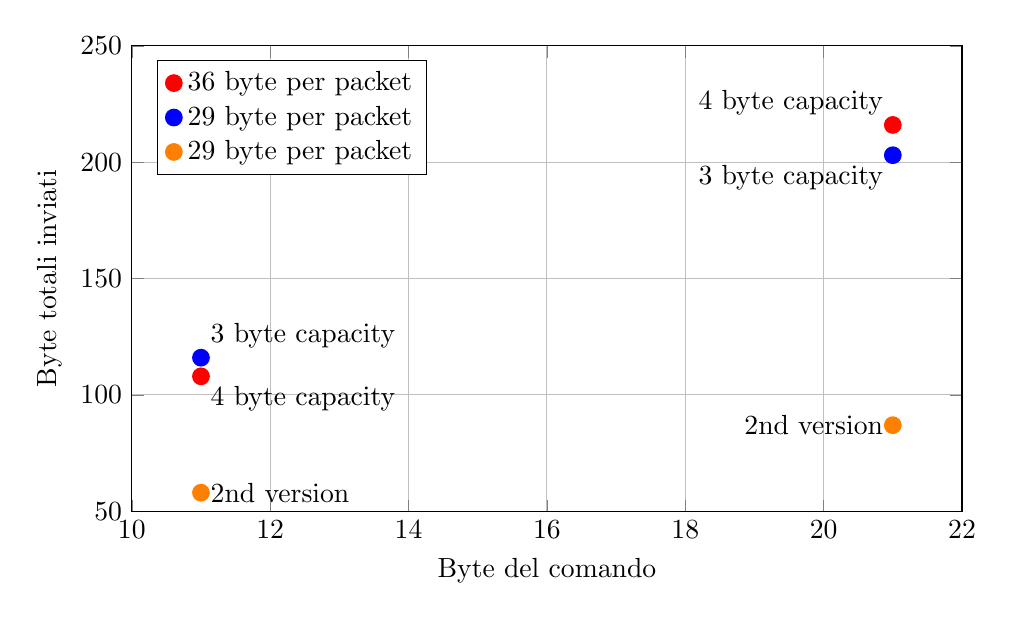
\begin{tikzpicture} 
    \tikzset{
    cmd11/.style={circle,fill=red,inner sep=2pt},
    cmd21/.style={circle,fill=blue,inner sep=2pt}
}
\begin{axis}[
    xlabel={Byte del comando}, 
    ylabel={Byte totali inviati},
    grid=major,
    width=\textwidth,
    height=0.618\textwidth, 
    domain=10:22,
    ymin=50,
    ymax=250, 
    legend pos=north west,
    legend entries={36 byte per packet, 29 byte per packet, 29 byte per packet}
]  
% Plot points
\addplot[only marks, mark=*, mark size=3pt, red] 
coordinates {(11,108) (21,216)};
\addplot[only marks, mark=*, mark size=3pt, blue] 
coordinates {(11,116) (21,203)}; 
\addplot[only marks, mark=*, mark size=3pt, orange] 
coordinates {(11,58) (21,87)}; 
% Add labels for the points 
\node[below right] at (axis cs:11,108) {4 byte capacity};
\node[above left] at (axis cs:21,216) {4 byte capacity};
\node[above right] at (axis cs:11,116) {3 byte capacity}; 
\node[below left] at (axis cs:21,203) {3 byte capacity}; 

\node[right] at (axis cs:11,58) {2nd version}; 
\node[left] at (axis cs:21,87) {2nd version}; 

\end{axis}
\end{tikzpicture}
\caption{Analisi tempi esecuzione \textit{Redirect}} 
\label{table:redirect:bytetotali:bytecomando}
\end{center}
Dall'analisi segue che il metodo \hyperref[redirect:casoB]{B} risulti il migliore. 
Non è facilmente rilevabile, siccome ripsetta gli standard definiti.  
Ciò risulta in un maggior numero di byte spediti per comandi corti mentre risulta un vantaggio per comandi di lunghezza maggiore. 
Infatti nel lungo periodo spedisce in totale un numero minore di byte rispetto alla sua controparte. 
\vspace{2ex} \newline 
Una possibile \textbf{alternativa} potrebbe essere quella di \textbf{usare il campo} \textit{gateway} e 
\textbf{strutturare il pacchetto} nella seconda maniera; 
e quindi evitando tutta la parte ICMP del datagram. 
Ciò porta la \textit{capacità del pacchetto} a \textbf{7 byte} e i\textit{ byte per pacchetto} a \textbf{29 byte}. 
I risultati si possono vedere nel grafico [Tabel:\ref{table:redirect:bytetotali:bytecomando} Arancione] 
\begin{center}
    Tuttavia questo approccio risulterà impossibile. 
    Il motivo è che questo campo viene usato attivamente per indicare all'host mittente un percorso migliore. 
    Ciò potrebbe portare a un ocntrollo di questo campo e alla scoperta della sua invalidità. 
    \footnote{Una pezza a questa cosa potrebbe usare solo l'utlimo byte per inserire i dati mentre i restanti per indicare l'indirizzo IP}
\end{center}

\subsubsection{Echo Request or Echo Reply Message (ICMPv4)} 
Nel protocollo \textbf{ICMPv4} la tipologia di messaggio \textit{Echo}, viene usata per ricevere indietro una risposta da un host. 
\vspace{1ex} \newline 
I dati ricevuti nel messaggio di Echo, devono essere restituiti nel messaggio di risposta. 
Inoltre i'identificatore e il numero di sequenza possono essere utilizzati dal 
mittente per facilitare l'abbinamento delle risposte con le richieste.
%Ad esempio, l'identificatore potrebbe essere utilizzato come una porta in TCP o UDP per identificare una 
%sessione e il numero di sequenza potrebbe essere incrementato a ogni richiesta di eco inviata.
Chi risponde alla richiesta Echo, restituisce gli stessi valori nella risposta. 
\vspace{2ex} \newline 
Per creare un messaggio di risposta, gli indirizzi di origine e di destinazione vengono semplicemente invertiti,
il codice da 8 viene modificato in 0 e il checksum viene ricalcolato. 

\subsubsection*{Struttura del pacchetto} 
\begin{bytefield}[bitwidth=1.1em]{32} 
    %\bitbox{8}{0} & \bitbox{8}{1} & \bitbox{8}{2} & \bitbox{8}{3} \\
    \bitheader{0-31} \\
    \bitbox{8}{Type (1B)} & \bitbox{8}{Code (1B)} & \bitbox{16}{Checksum (2B)} \\
    \bitbox{16}{Identifier (2B)} && \bitbox{16}{Sequence Number (2B)} \\
    \bitbox{32}{Data ... ($\geq$ 0B)} 
\end{bytefield}
I campi sono i seguenti: 
\begin{itemize}
    \item Type: 8 per i messaggi Echo Request; 0 per i messaggi Echo Reply.
    \item Code: 0 
    \item Checksum: è il complemento a 16 bit del complemento a uno relativo alla somma del messaggio ICMP 
    (che inizia con il campo Type). Verrà calcolato se il campo è zero. 
    \item Identifier: se il codice = 0; l'identificatore serve per facilitare la corrispondenza tra le richieste Echo e le Risposte Echo. Può essere zero. 
    \item Sequence Number: se il codice = 0; il numero di sequenza serve per facilitare la corrispondenza tra le richieste Echo e le Risposte Echo. Può essere zero. 
\end{itemize}
\vspace{1ex} 
Si sfrutteranno quindi i campi nel seguente modo: 
\begin{itemize}
    \item Il campo \textbf{checksum} non è utilizzabile. 
    Essendo il complemento ad 1 del contenuto del pacchetto, se non combaciasse il pacchetto verrebbe scartato. 
    \item Il campo \textbf{identifier} che siccome serve a definire un identificativo delle richieste, può essere un qualsiasi valore. 
    \item Il campo di \textbf{sequenza} potrebbe essere utilizzato per inserire le informazioni; 
    tuttavia, dalle specifiche \href{https://www.rfc-editor.org/rfc/rfc792.html#:~:text=Echo%20or%20Echo%20Reply%20Message}{RFC 792}, esso viene incrementato ad ogni richiesta inviata. 
    Quindi se il valore del campo è troppo variabile, potrebbe risultare sospetto. 
\end{itemize}

\subsubsection*{Analisi complessiva} 
Per l'analisi supponiamo di mandare due comandi che sono: 
\begin{itemize}
    \item \textbf{echo 'Ciao'}: che sono \textit{11 byte} (e quindi \textit{88 bit}\footnote{\label{note:echo:analisi}Ciò sarà utile per i \textit{Timing Covert Channel}})
    \item \textbf{cd /home/marco; ls -l}: che sono \textit{21 byte}  (e quindi \textit{168 bit}\textsuperscript{\ref{note:echo:analisi}}) %\footnotemark[2]
\end{itemize}
Sappiamo che nel caso migliore la capacità di trasmissione di ogni pacchetto è \textbf{2 byte} \label{echo:casoA}; 
questo perchè il campo \textit{identifier} ha una lunghezza di soli \textit{2 byte}. %20
\begin{itemize}
    \item Ogni pacchetto del caso (che chiameremo \hyperref[echo:casoA]{A}) trasporterà \textbf{8 byte}
    \footnote{8 per i campi ICMP presenti}
    (supponendo che non si inseriscano dati) 
\end{itemize} 
Ora si analizza quanti pacchetti saranno necessari per inviare i comandi. \newline
Nel caso si mandasse il comando \textbf{echo 'Ciao'} il numero di pacchetti necessari sarebbere: 
\begin{itemize}
    \item Caso \hyperref[echo:casoA]{A}: Sarebbero necessari \textit{6 pacchetti}. 
    E quindi siccome ogni pacchetto trasporta \textit{8 byte}; si spediranno in totale \textbf{48 byte}. 
\end{itemize} 
Ora analiziamo il comando \textbf{cd /home/marco; ls -l} e quanti pacchetti saranno necessari: 
\begin{itemize}
    \item Caso \hyperref[echo:casoA]{A}: siccome è di \textit{21 byte}, servirebbero \textit{11 pacchetti}. 
    Quindi siccome ogni pacchetto trasporta \textit{8 byte}; si spediranno in totale \textbf{88 byte}. 
\end{itemize}

\begin{center} 
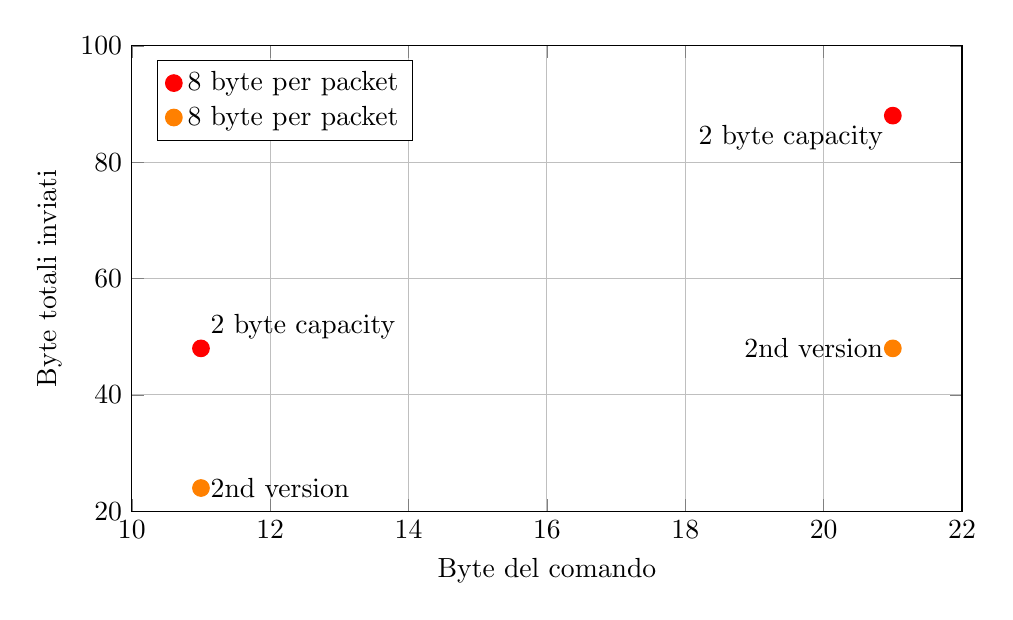
\begin{tikzpicture} 
    \tikzset{
    cmd11/.style={circle,fill=red,inner sep=2pt},
    cmd21/.style={circle,fill=blue,inner sep=2pt}
}
\begin{axis}[
    xlabel={Byte del comando}, 
    ylabel={Byte totali inviati},
    grid=major,
    width=\textwidth,
    height=0.618\textwidth, 
    domain=10:22,
    ymin=20,
    ymax=100, 
    legend pos=north west,
    legend entries={8 byte per packet, 8 byte per packet}
]  
% Plot points
\addplot[only marks, mark=*, mark size=3pt, red] 
coordinates {(11,48) (21,88)}; 
\addplot[only marks, mark=*, mark size=3pt, orange] 
coordinates {(11,24) (21,48)}; 
% Add labels for the points 
\node[above right] at (axis cs:11,48) {2 byte capacity}; 
\node[below left] at (axis cs:21,88) {2 byte capacity}; 

\node[right] at (axis cs:11,24) {2nd version}; 
\node[left] at (axis cs:21,48) {2nd version}; 

\end{axis}
\end{tikzpicture}
\caption{Analisi tempi esecuzione \textit{Echo}} 
\label{table:echo:bytetotali:bytecomando}
\end{center}
Dall'analisi segue che il metodo \hyperref[echo:casoA]{A} non riuslta il migliore. 
Infatti analizzando il caso in cui si usasse anche il campo di \textit{sequenza} [Tabella:\ref{table:echo:bytetotali:bytecomando} Arancione]; 
si avrà una notevole differenza di bytes spediti totalmente rispetto al caso \hyperref[echo:casoA]{A}. 
Tuttavia siccome l'uso di questo campo comporta una maggiore visibilità, 
si sceglie di non usarlo e correre il rischio. Questo comporterà l'invio di un maggior numero di bytes; 
che anche ciò potrebbe rivelare il Covert Channel. 
\vspace{1ex} \newline 
Si è scelto quindi di usare il metodo \hyperref[echo:casoA]{A} ed affidarsi ai meccanismi di difesa presenti nella vittima; 
nella speranza che un numero elevato di pacchetti, ma senza il campo \textit{dati}, possano essere considerati innocqui.
\vspace{2ex} \newline 
Un \textbf{metodo maggiormente efficace} è proprio l'uso del campo \textbf{data}. 
Tuttavia anche questo approccio potrebbe destare sospetti. 
Infatti si dovrà decidere se mandare i dati in chiaro o cifrati:
\begin{itemize}
    \item Nel primo caso sarà possibile leggerne il contenuto. 
    \item Nell'altro, invece, la non possibilità di leggerne il ocntenuto rende lo scambio sospetto. 
    Siccome esistono canali migliori per poter scambiare informazioni in questo modo. 
\end{itemize} 
Inoltre bisognerebbe calcolare la capacità minima afifnche questo campo non risulti anomalo, ma sicuramente sarà maggiore di 2 byte. 
Questo lo si può affermare dopo aver testato i programmi di ping sia su Linux che su Windows. 

\subsubsection{Timestamp or Timestamp Reply Message (ICMPv4)} 
Nel protocollo \textbf{ICMPv4} la tipologia di messaggio \textit{Timestamp}, viene usata per ricevere indietro una risposta da un host. 
\vspace{1ex} \newline 
L'identificatore e il numero di sequenza possono essere utilizzati dal mittente del pacchetto per facilitare l'abbinamento delle risposte con le richieste.
%Ad esempio, l'identificatore potrebbe essere utilizzato come una porta in TCP o UDP per identificare una sessione e il numero di sequenza potrebbe essere incrementato a ogni richiesta inviata.
%La destinazione restituisce gli stessi valori nella risposta. 
Inoltre i dati ricevuti nel messaggio di richiesta, vengono restituiti in quello di risposta insieme a dei timestamp aggiuntivi. 
Il timestamp è pari a 32 bit e indica i millisecondi che sono passati dalla mezzanotte UT.
%Un utilizzo di questi timestamp è descritto da Mills [5].
\vspace{1ex} \newline 
Se l'ora non è disponibile in millisecondi o non può essere fornita rispetto alla mezzanotte UT, 
è possibile inserire qualsiasi ora in un timestamp, a condizione che anche il bit di ordine superiore del 
timestamp sia impostato per indicare questo valore non standard. 
\vspace{1ex} \newline  
In un messaggio di risposta, l'indirizzo della sorgente sarà la destinazione. 
Quindi per poter creare un messaggio di risposta timestamp, gli indirizzi di sorgente e destinazione vengono semplicemente invertiti, il codice di tipo viene modificato in 14 e il checksum viene ricalcolato.

\subsubsection*{Struttura del pacchetto} 
\begin{bytefield}[bitwidth=1.1em]{32} 
    %\bitbox{8}{0} & \bitbox{8}{1} & \bitbox{8}{2} & \bitbox{8}{3} \\
    \bitheader{0-31} \\
    \bitbox{8}{Type (1B)} & \bitbox{8}{Code (1B)} & \bitbox{16}{Checksum (2B)} \\
    \bitbox{16}{Identifier (2B)} && \bitbox{16}{Sequence Number (2B)} \\ 
    \bitbox{32}{Originate Timestamp (4B)} \\
    \bitbox{32}{Receive Timestamp (4B)} \\
    \bitbox{32}{Transmit Timestamp (4B)} \\
    \bitbox{32}{Data ... ($\geq$ 0B)} 
\end{bytefield}
I campi sono i seguenti: 
\begin{itemize}
    \item Type: 13 per i messaggi Timestamp Request; 14 per i messaggi Timestamp Reply.
    \item Code: 0 può essere ricevuto da un gateway o da un host
    \item Checksum: è il complemento a 16 bit del complemento a uno relativo alla somma del messaggio ICMP 
    (che inizia con il campo Type). Verrà calcolato se il campo è zero. 
    \item Identifier: se il codice = 0; l'identificatore serve per facilitare la corrispondenza tra le richieste Echo e le Risposte Echo. Può essere zero. 
    \item Sequence Number: se il codice = 0; il numero di sequenza serve per facilitare la corrispondenza tra le richieste Echo e le Risposte Echo. Può essere zero. 
    \item Originate Timestamp: tempo in cui il mittente ha toccato il messaggio per l'ultima volta prima di inviarlo. 
    \item Receive Timestamp: tempo in cui il destinatario ha toccato per la prima volta il messaggio (alla ricezione). 
    \item Transmit Timestamp: tempo in cui il destinatario ha toccato il messaggio per l'ultima volta prima di inviarlo. 
\end{itemize}  
Si sfrutteranno quindi i campi nel seguente modo: 
\begin{itemize}
    \item Il campo \textbf{checksum} non è utilizzabile. 
    Essendo il complemento ad 1 del contenuto del pacchetto, se non combaciasse il pacchetto verrebbe scartato. 
    \item Il campo \textbf{identifier} che siccome serve a definire un identificativo delle richieste, può essere un qualsiasi valore. 
    \item Il campo di \textbf{sequenza} potrebbe essere utilizzato per inserire le informazioni; 
    tuttavia, dalle specifiche \href{https://www.rfc-editor.org/rfc/rfc792.html#:~:text=Timestamp%20or%20Timestamp%20Reply%20Message}{RFC 792}, esso viene incrementato ad ogni richiesta inviata. %%20 
    Quindi se il valore del campo è troppo variabile, potrebbe risultare sospetto. 
    \item I campi \textbf{originate timestamp}, \textbf{receive timestamp}, \textbf{transmit timestamp} dovranno contenere solo il tempo in milliseocndi dalla mezzanotte UT. 
    Quindi in ognuno dei campi può essere inserito un byte nella parte indicante i millisecondi. 
    Si potrebbero inserire un numero magigore di dati sfruttando l'intera lunghezza dei campi ma poi i tempi non risulterebbero congruenti fra di loro
    \footnote{Si potrebbe avere il caso che il destinatario ha modificato il messagio prima di poterlo ricevere}
\end{itemize}

\subsubsection*{Analisi complessiva} 
Per l'analisi supponiamo di mandare due comandi che sono: 
\begin{itemize}
    \item \textbf{echo 'Ciao'}: che sono \textit{11 byte} (e quindi \textit{88 bit}\footnote{\label{note:timestamp:analisi}Ciò sarà utile per i \textit{Timing Covert Channel}})
    \item \textbf{cd /home/marco; ls -l}: che sono \textit{21 byte}  (e quindi \textit{168 bit}\textsuperscript{\ref{note:timestamp:analisi}}) %\footnotemark[2]
\end{itemize}
Sappiamo che nel caso migliore la capacità di trasmissione di ogni pacchetto è \textbf{5 byte} \label{timestamp:casoA}; 
questo perchè il campo \textit{identifier} ha una lunghezza di \textit{2 byte} mentre i tre campi timestamp contengono \textit{un byte} ciascuno. %20
\begin{itemize}
    \item Ogni pacchetto del caso (che chiameremo \hyperref[timestamp:casoA]{A}) trasporterà \textbf{20 byte} 
    \footnote{20 per i campi ICMP} 
\end{itemize} 
Ora si analizza quanti pacchetti saranno necessari per inviare i comandi. \newline
Nel caso si mandasse il comando \textbf{echo 'Ciao'} il numero di pacchetti necessari sarebbere: 
\begin{itemize}
    \item Caso \hyperref[timestamp:casoA]{A}: Sarebbero necessari \textit{3 pacchetti}. 
    E quindi siccome ogni pacchetto trasporta \textit{20 byte}; si spediranno in totale \textbf{60 byte}. 
\end{itemize} 
Ora analiziamo il comando \textbf{cd /home/marco; ls -l} e quanti pacchetti saranno necessari: 
\begin{itemize}
    \item Caso \hyperref[timestamp:casoA]{A}: siccome è di \textit{21 byte}, servirebbero \textit{5 pacchetti}. 
    Quindi siccome ogni pacchetto trasporta \textit{20 byte}; si spediranno in totale \textbf{100 byte}. 
\end{itemize}

\begin{center} 
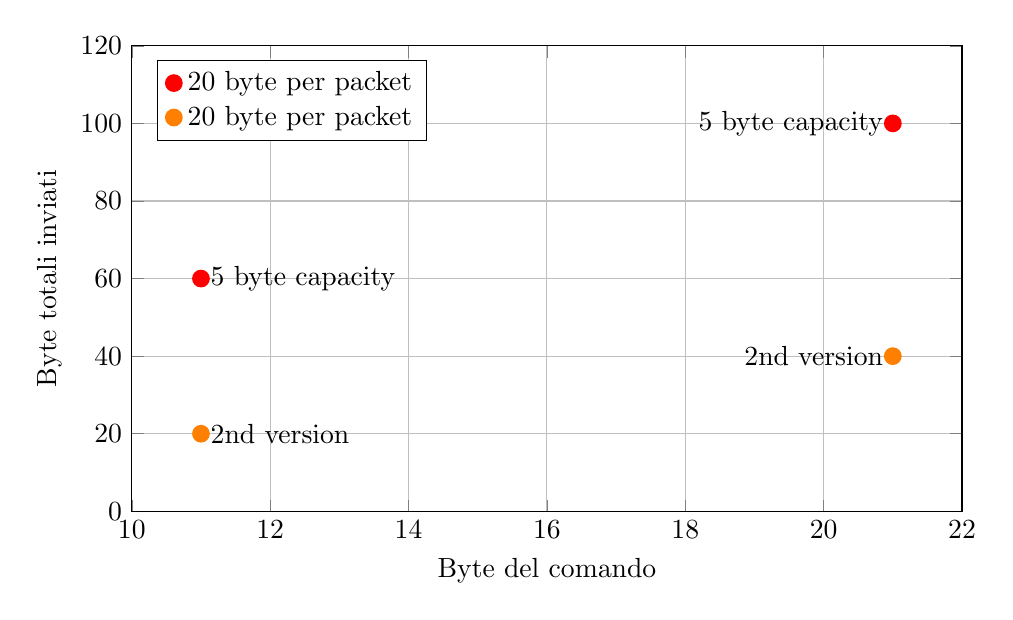
\begin{tikzpicture} 
    \tikzset{
    cmd11/.style={circle,fill=red,inner sep=2pt},
    cmd21/.style={circle,fill=blue,inner sep=2pt}
}
\begin{axis}[
    xlabel={Byte del comando}, 
    ylabel={Byte totali inviati},
    grid=major,
    width=\textwidth,
    height=0.618\textwidth, 
    domain=10:22,
    ymin=0,
    ymax=120, 
    legend pos=north west,
    legend entries={20 byte per packet, 20 byte per packet}
]  
% Plot points
\addplot[only marks, mark=*, mark size=3pt, red] 
coordinates {(11,60) (21,100)}; 
\addplot[only marks, mark=*, mark size=3pt, orange] 
coordinates {(11,20) (21,40)}; 
% Add labels for the points 
\node[right] at (axis cs:11,60) {5 byte capacity}; 
\node[left] at (axis cs:21,100) {5 byte capacity}; 

\node[right] at (axis cs:11,20) {2nd version}; 
\node[left] at (axis cs:21,40) {2nd version}; 

\end{axis}
\end{tikzpicture}
\caption{Analisi tempi esecuzione \textit{Timestamp}} 
\label{table:timestamp:bytetotali:bytecomando}
\end{center}  
Dall'analisi segue che il metodo \hyperref[echo:casoA]{A} non riuslta il migliore. 
Infatti analizzando il caso in cui si usasse anche l'intera dimesnione dei campi \textit{timestamp} [Tabella:\ref{table:timestamp:bytetotali:bytecomando} Arancione]; 
si avrà una notevole differenza di bytes spediti totalmente rispetto alla controparte
\footnote{Questo perchè porta la capacitò del pacchetto a \textit{5 bytes} a \textbf{14 bytes}}. 
Tuttavia l'uso di questi campi risulta non possibile siccome le ore, i minuti e i secondi hanno un range di valori accettati e no
\footnote{I secondi, come i minuti devono essere compresi fra 0 e 59 mentre le ore fra 0 e 23}. 
Questo porta all'impossibilità di inserimento di alcune informazioni. 
In particoalre limita la possibilità di usare i caratteri il cui codice ASCII non è compreso nel range.   
\vspace{1ex} \newline
Una modifica per risolvere la cosa è l'inserimento diretto diretto nel campo. 
Tuttavia questo porterà a valori di tempo scostanti: 
\begin{lstlisting}[
    language=Python, basicstyle=\tiny, firstnumber=0, numbers=left, numberstyle=\tiny, xleftmargin=5mm
    %
    ,emph={data}, emphstyle=\color{red} 
    ,emph={[2]index},emphstyle={[2]\color{blue}} 
    ,emph={[3]}, emphstyle={[3]\color{olive}} 
    ,literate={.}{{\char46}}1 {:}{{\char58}}1 
] 
data="echo 'Ciao'".encode() 
for index in range(0, len(data), 12): 
    print(f"Byte data: {int.from_bytes(data[index:index+4])}")
    print(f"Byte data: {int.from_bytes(data[index+5:index+8])}") 
    print(f"Byte data: {int.from_bytes(data[index+8:index+12])}") 
\end{lstlisting} 
\label{code:timestamp:casoB}
\captionof{lstlisting}{Si usa l'intero Timestamp per i dati}
\begin{lstlisting} [
    language=Python, basicstyle=\tiny, firstnumber=0, numbers=left, numberstyle=\tiny, xleftmargin=5mm
    %
    ,emph={data, icmp_ts_ori, icmp_ts_rx, icmp_ts_tx}, emphstyle=\color{red} 
    ,emph={[2]index, data_pkt},emphstyle={[2]\color{blue}} 
    ,emph={[3]current_time, midnight}, emphstyle={[3]\color{olive}} 
    ,literate={.}{{\char46}}1 {:}{{\char58}}1 
] 
#Output 
Byte data: 1701013615
Byte data: 2573161
Byte data: 6385447
\end{lstlisting} 
\label{code:timestamp:casoB:output}
\captionof{lstlisting}{Output del codice} 
\vspace{1ex} 
Ciò risulta sconveniente siccome, per come si sono definiti i campi di timestamp, questi tempi dovrebbero essere l'uno il successivo dell'altro. 
\vspace{2ex} \newline 
Questo limite non è presente nel campo \textit{milliseocndi} siccome il suo intervallo arriva sino a \href{https://docs.python.org/3.11/library/datetime.html#datetime.datetime.microsecond}{1000}. 
Inserendo un singolo byte il massimo valore inseribile è $2^8-1=255$. 
Il che copre tutti i possibili caratteri possibili, siccome in ASCII ognuno di essi è un singolo byte. 
\vspace{1ex} \newline 
Si procede quindi sulla strada del caso \hyperref[timestamp:casoA]{A} ricavando dal byte da inserire, l'intero risultante e poi lo si moltiplica per $10^3$.
Quest'ultimo valore sarà quello che si inserirà nel campo \textit{millisecondi}. 
Dopodichè una volta definito il timestamp, si noterà che in esso gli ultimi tre deciamli finali contengono il carattere inserito (\href{https://www.ascii-code.com/it}{espresso in decimale}). 
\vspace{1ex} \newline
\begin{lstlisting}[
    language=Python, basicstyle=\tiny, firstnumber=0, numbers=left, numberstyle=\tiny, xleftmargin=5mm
    %
    ,emph={data, icmp_ts_ori, icmp_ts_rx, icmp_ts_tx}, emphstyle=\color{red} 
    ,emph={[2]index, data_pkt},emphstyle={[2]\color{blue}} 
    ,emph={[3]current_time, midnight}, emphstyle={[3]\color{olive}} 
    ,literate={.}{{\char46}}1 {:}{{\char58}}1 
] 
data="echo 'Ciao'".encode() 
for index in range(0, len(data), 12): 
    icmp_id=icmp_id=(data[index]<<8)+data[index+1] 

    current_time=datetime.datetime.now(datetime.timezone.utc) 
    midnight = current_time.replace(
        hour=0, minute=0, second=0, microsecond=0
    ) 

    data_pkt=int.from_bytes(data[index+2:index+3]) *10**3
    current_time=current_time.replace(microsecond=data_pkt)
    icmp_ts_ori=int((current_time - midnight).total_seconds() * 1000) 
    print(f"Byte data: {data[index+2:index+3]}")
    print(f"Data pkt: {data_pkt}")
    print(f"Timestamp: {icmp_ts_ori}") 
    
    data_pkt=int.from_bytes(data[index+3:index+4]) *10**3 
    if current_time.second+1<60:
        current_time=current_time.replace(
            second=current_time.second+1, microsecond=data_pkt
        ) 
    else:
        current_time=current_time.replace(
            minute=current_time.minute+1
            ,second=(current_time.second+1)%60
            , microsecond=data_pkt
        ) 
    icmp_ts_rx=int((current_time - midnight).total_seconds() * 1000) 
    print(f"Byte data: {data[index+3:index+4]}")
    print(f"Data pkt: {data_pkt}")
    print(f"Timestamp: {icmp_ts_rx}") 

    data_pkt=int.from_bytes(data[index+4:index+5]) *10**3 
    if current_time.second+1<60: 
        current_time=current_time.replace(
            second=current_time.second+1, microsecond=data_pkt
        )
    else: 
        current_time=current_time.replace(
            minute=current_time.minute+1
            ,second=(current_time.second+1)%60
            ,microsecond=data_pkt
        )
    icmp_ts_tx=int((current_time - midnight).total_seconds() * 1000) 
    print(f"Byte data: {data[index+4:index+5]}")
    print(f"Data pkt: {data_pkt}")
    print(f"Timestamp: {icmp_ts_tx}")
\end{lstlisting} 
\label{code:timestamp:casoA}
\captionof{lstlisting}{Si usa un byte del Timestamp per i dati}
\begin{lstlisting} [
    language=Python, basicstyle=\tiny, firstnumber=0, numbers=left, numberstyle=\tiny, xleftmargin=5mm
    %
    ,emph={data, icmp_ts_ori, icmp_ts_rx, icmp_ts_tx}, emphstyle=\color{red} 
    ,emph={[2]index, data_pkt},emphstyle={[2]\color{blue}} 
    ,emph={[3]current_time, midnight}, emphstyle={[3]\color{olive}} 
    ,literate={.}{{\char46}}1 {:}{{\char58}}1 
] 
#Output 
ICMP id: 25955
Byte data: b'h'
    Data pkt: 104000
    Timestamp ori: 38494104
Byte data: b'o'
    Data pkt: 111000
    Timestamp rx: 38495111
Byte data: b' '
    Data pkt: 32000
    Timestamp tx: 38496032
ICMP id: 10051
Byte data: b'i'
    Data pkt: 105000
    Timestamp ori: 38494105
Byte data: b'a'
    Data pkt: 97000
    Timestamp rx: 38495097
Byte data: b'o'
    Data pkt: 111000
    Timestamp tx: 38496111
ICMP id: 9984
\end{lstlisting} 
\label{code:timestamp:casoA:output}
\captionof{lstlisting}{Output del codice}

\subsubsection{Information Request or Information Reply Message (ICMPv4)} 
Nel protocollo \textbf{ICMPv4} la tipologia di messaggio \textit{Information}, viene usata per consentire a un host di scoprire il numero della rete in cui si trova. 
E quindi per capire se si trova nella stesse rete dell'host che risponde. 
L'identificatore e il numero di sequenza possono essere utilizzati dal mittente del pacchetto per facilitare l'abbinamento delle risposte con le richieste.
\vspace{1ex} \newline 
Questo messaggio può essere inviato con la rete sorgente nel campo mittente e 
la destinazione nell'intstazione IP pari a zero (ciò significa "questa" rete). 
Tuttavia l'intestazione IP presente nel messaggio di risposta dovrà essere inviata con gli indirizzi IP completamente specificati.
\vspace{2ex} \newline 
Per creare un messaggio di risposta, gli indirizzi di origine e di destinazione vengono invertiti,
il codice da 15 viene modificato in 16 e il checksum viene ricalcolato. 

\subsubsection*{Struttura del pacchetto} 
\begin{bytefield}[bitwidth=1.1em]{32} 
    %\bitbox{8}{0} & \bitbox{8}{1} & \bitbox{8}{2} & \bitbox{8}{3} \\
    \bitheader{0-31} \\
    \bitbox{8}{Type (1B)} & \bitbox{8}{Code (1B)} & \bitbox{16}{Checksum (2B)} \\
    \bitbox{16}{Identifier (2B)} && \bitbox{16}{Sequence Number (2B)} 
\end{bytefield}
I campi sono i seguenti: 
\begin{itemize}
    \item Type: 15 per i messaggi Information Request; 16 per i messaggi Information Reply. 
    \item Code: 0 che può essere ricevuto sia da un gateway che da un host
    \item Checksum: è il complemento a 16 bit del complemento a uno relativo alla somma del messaggio ICMP 
    (che inizia con il campo Type). Verrà calcolato se il campo è zero. 
    \item Identifier: se il codice = 0; l'identificatore serve per facilitare la corrispondenza tra le richieste Echo e le Risposte Echo. Può essere zero. 
    \item Sequence Number: se il codice = 0; il numero di sequenza serve per facilitare la corrispondenza tra le richieste Echo e le Risposte Echo. Può essere zero. 
\end{itemize}
\vspace{1ex} 
Si sfrutteranno quindi i campi nel seguente modo: 
\begin{itemize}
    \item Il campo \textbf{checksum} non è utilizzabile. 
    Essendo il complemento ad 1 del contenuto del pacchetto, se non combaciasse il pacchetto verrebbe scartato. 
    \item Il campo \textbf{identifier} che siccome serve a definire un identificativo delle richieste, può essere un qualsiasi valore. 
    \item Il campo di \textbf{sequenza} potrebbe essere utilizzato per inserire le informazioni; 
    tuttavia, dalle specifiche \href{https://www.rfc-editor.org/rfc/rfc792.html#:~:text=Information%20Request%20or%20Information%20Reply%20Message}{RFC 792}, esso viene incrementato ad ogni richiesta inviata. %20
    Quindi se il valore del campo sarà troppo variabile, potrebbe risultare sospetto. 
\end{itemize} 

\subsubsection*{Analisi complessiva} 
Per l'analisi supponiamo di mandare due comandi che sono: 
\begin{itemize}
    \item \textbf{echo 'Ciao'}: che sono \textit{11 byte} (e quindi \textit{88 bit}\footnote{\label{note:information:analisi}Ciò sarà utile per i \textit{Timing Covert Channel}})
    \item \textbf{cd /home/marco; ls -l}: che sono \textit{21 byte}  (e quindi \textit{168 bit}\textsuperscript{\ref{note:information:analisi}}) %\footnotemark[2]
\end{itemize}
Sappiamo che nel caso migliore la capacità di trasmissione di ogni pacchetto è \textbf{2 byte} \label{information:casoA}; 
questo perchè il campo \textit{identifier} ha una lunghezza di soli \textit{2 byte}. %20 
\begin{itemize}
    \item Ogni pacchetto del caso (che chiameremo \hyperref[information:casoA]{A}) trasporterà \textbf{8 byte}
    \footnote{8 per i campi ICMP} 
\end{itemize} 
Ora si analizza quanti pacchetti saranno necessari per inviare i comandi. \newline
Nel caso si mandasse il comando \textbf{information 'Ciao'} il numero di pacchetti necessari sarebbere: 
\begin{itemize}
    \item Caso \hyperref[information:casoA]{A}: Sarebbero necessari \textit{6 pacchetti}. 
    E quindi siccome ogni pacchetto trasporta \textit{8 byte}; si spediranno in totale \textbf{48 byte}. 
\end{itemize} 
Ora analiziamo il comando \textbf{cd /home/marco; ls -l} e quanti pacchetti saranno necessari: 
\begin{itemize}
    \item Caso \hyperref[information:casoA]{A}: siccome è di \textit{21 byte}, servirebbero \textit{11 pacchetti}. 
    Quindi siccome ogni pacchetto trasporta \textit{8 byte}; si spediranno in totale \textbf{88 byte}. 
\end{itemize}

\begin{center} 
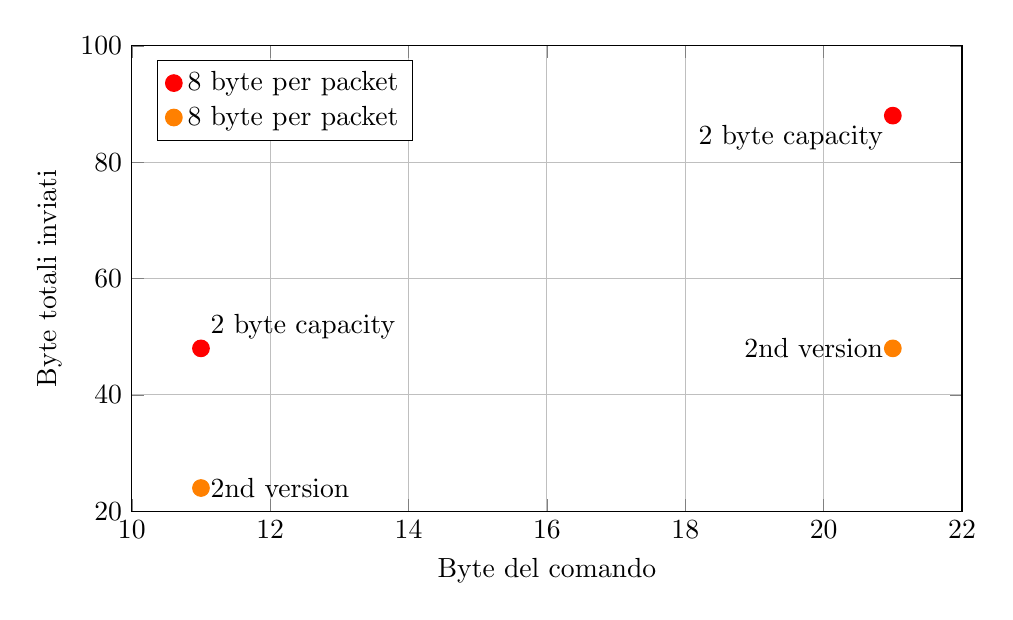
\begin{tikzpicture} 
    \tikzset{
    cmd11/.style={circle,fill=red,inner sep=2pt},
    cmd21/.style={circle,fill=blue,inner sep=2pt}
}
\begin{axis}[
    xlabel={Byte del comando}, 
    ylabel={Byte totali inviati},
    grid=major,
    width=\textwidth,
    height=0.618\textwidth, 
    domain=10:22,
    ymin=20,
    ymax=100, 
    legend pos=north west,
    legend entries={8 byte per packet, 8 byte per packet}
]  
% Plot points
\addplot[only marks, mark=*, mark size=3pt, red] 
coordinates {(11,48) (21,88)}; 
\addplot[only marks, mark=*, mark size=3pt, orange] 
coordinates {(11,24) (21,48)}; 
% Add labels for the points 
\node[above right] at (axis cs:11,48) {2 byte capacity}; 
\node[below left] at (axis cs:21,88) {2 byte capacity}; 

\node[right] at (axis cs:11,24) {2nd version}; 
\node[left] at (axis cs:21,48) {2nd version}; 

\end{axis}
\end{tikzpicture}
\caption{Analisi tempi esecuzione \textit{Information}} 
\label{table:information:bytetotali:bytecomando}
\end{center}
Dall'analisi segue che il metodo \hyperref[information:casoA]{A} non riuslta il migliore. 
Infatti analizzando il caso in cui si usasse anche il campo di \textit{sequenza} [Tabella:\ref{table:information:bytetotali:bytecomando} Arancione]; 
si avrà una notevole differenza di bytes spediti totalmente rispetto al caso \hyperref[information:casoA]{A}. 
\vspace{1ex} \newline
Tuttavia siccome l'uso di questo campo comporta una maggiore visibilità, 
si sceglie di non usarlo e correre il rischio. 
Questo comporterà l'invio di un maggior numero di bytes; 
che anche ciò potrebbe rivelare il Covert Channel. 
\vspace{1ex} \newline 
Si è scelto quindi di usare il metodo \hyperref[information:casoA]{A} ed affidarsi ai meccanismi di difesa presenti nella vittima; 
nella speranza che un numero elevato di pacchetti possano essere considerati innocqui.


\subsubsection{Destination Unreachable Message (ICMPv6)} 
Nel protocollo \textbf{ICMPv6} la tipologia di messaggio \textit{Destination Unreachable}, 
viene generato da un router (o dal livello IPv6 nel nodo di origine) in risposta a un pacchetto che non può essere recapitato 
(alla sua destinazione) per motivi diversi dalla congestione. 
Un messaggio ICMPv6 non verrà (e non dovrà) generato se un pacchetto viene scartato a causa della congestione del traffico. 
\vspace{1ex} \newline 
I codici associati ai possibili casi sono i seguenti: 
\begin{itemize}
    \item[0] quando il motivo della mancata consegna, è la mancanza di una voce corrispondente nella tabella di 
    routing. 
    %(L'errore può verificarsi in nodi che non contengono una "rotta predefinita" nelle tabelle di routing)
    \item[1] il motivo della mancata consegna è relativo ad un divieto amministrativo (ad esempio, un "filtro firewall")
    \item[2] il motivo della mancata consegna è che la destinazione è al di fuori della visuale 
    \footnote{\textbf{Scope}: ambito, ambiente, visuale, raggio d'azione} del mittente. 
    Questa condizione può verificarsi solo quando la visione dell'indirizzo mittente è inferiore a quello del destinatario 
    (ad esempio, quando un pacchetto ha un indirizzo mittente link-locale e un indirizzo di destinazione global-scope) 
    e il pacchetto non può essere consegnato senza uscire dall'ambito dell'indirizzo sorgente.
    \item[3] il motivo del mancato recapito non rientra in nessuno degli altri codici.  
    %Example of such cases are an inability to resolve the IPv6 destination address into a corresponding link address, or a link-specific problem of some sort.
    %Esempi di tali casi sono l'impossibilità di risolvere l'indirizzo di destinazione IPv6 in un indirizzo di collegamento corrispondente o un problema specifico del collegamento. 
    \item[4] quando un pacchetto in cui il protocollo di trasporto (ad esempio, UDP) non ha un listener, e 
    se tale protocollo di trasporto non ha di mezzi alternativi per informare il mittente della cosa. 
    In questi casi è il nodo di destinazione a generare il messaggio \textit{Destination Unreachable} in risposta all'evento. 
    \item[5] il motivo del mancato recapito è che il pacchetto non è consentito a causa dei criteri delle politiche di filtraggio (sia in ingresso o in uscita). 
    \item[6] il motivo del mancato recapito è che il percorso verso la destinazione è un percorso rifiutato. 
    Ciò può verificarsi se il router è stato configurato per rifiutare il traffico verso uno specifico indirizzo, prefisso o sottorete. 
\end{itemize}
%One specific case in which a Destination Unreachable message is sent with a code 3 is in response to a packet received by a router from a point-to-point link, destined to an address within a subnet assigned to that same link (other than one of the receiving router's own addresses).  In such a case, the packet MUST NOT be forwarded back onto the arrival link. 
%Codes 5 and 6 are more informative subsets of code 1. 
%For security reasons, it is recommended that implementations SHOULD allow sending of ICMP destination unreachable messages to be disabled, preferably on a per-interface basis.
\vspace{1ex} 
%\textbf{Notifica al livello superiore} \newline
Un nodo che riceve un messaggio ICMPv6 \textit{Destination Unreachable} deve notificare la cosa al 
processo di livello superiore (se il processo in questione può essere identificato).

\subsubsection*{Struttura del pacchetto} 
\begin{bytefield}[bitwidth=1.1em]{32} 
    %\bitbox{8}{0} & \bitbox{8}{1} & \bitbox{8}{2} & \bitbox{8}{3} \\
    \bitheader{0-31} \\
    \bitbox{8} {Type (1B)} & \bitbox{8}{Code (1B)} & \bitbox{16}{Checksum (2B)} \\
    \bitbox{32} {Unused (4B)} \\
    \bitbox{32} {As much of invoking packet as possible without} \\
    \bitbox{32} {the ICMPv6 packet exceeding the minimum IPv6 MTU ($\geq$ 0B)} 
\end{bytefield}
I campi sono i seguenti: 
\begin{itemize}
    \item Type: 1
    \item Code: 0-6 
    \item Checksum: è il complemento a 16 bit del complemento a uno relativo alla somma del messaggio ICMP 
    (che inizia con il campo Type). Verrà calcolato se il campo è zero. 
    \item Unused: il campo non è utilizzato per tutti i codici possibili.
    Deve essere inizializzato a zero dal mittente e ignorato dal destinatario. 
    \item Invoking Packet: quanta parte del pacchetto (che ha attivato l'errore ICMPv6) debba essere inclusa. 
    Il tutto senza eccedere il \textit{IPv6 MTU} che equivale a \href{https://www.rfc-editor.org/rfc/rfc2460#section-5}{\textbf{1280 bytes}}. 
    \footnote{\textbf{MTU}=maximum transmission unit ovvero il massimo carico possibile} 
    \footnote{L'\textit{intestazione IP} contiene al minimo 40 byte} 
\end{itemize}
%IPv6 richiede che ogni link su internet abbia un MTU di 1280 ottetti o più. 
%Su ogni link che non può portare pacchetti da 1280 ottetti in un solo pezzo, 
%debbono essere previste frammentazione e riassemblaggio specifici al link, ad un livello inferiore ad IPv6. 
%Questo significa che in questo caso la frammentazione avviene a livello link layer, 
%non viene in nessun modo gestita da IPv6 (a livello rete) ed è del tutto trasparente.
\vspace{1ex} 
Si sfrutteranno quindi i campi nel seguente modo: 
\begin{itemize}
    \item Il campo \textbf{checksum} non è utilizzabile. 
    Essendo il complemento ad 1 del contenuto del pacchetto, se non combaciasse il pacchetto verrebbe scartato. 
    \item Il campo \textbf{unused} dalle specifiche \href{https://www.rfc-editor.org/rfc/rfc4443#section-3.1}{RFC 4434} dovrebbe essere 0. 
    Tuttavia nel nostro caso è stato utilizzato per testare la presenza della \textit{Deep Packet Inspection}. 
    \item Nel campo \textbf{Invoking Packet} si userà il campo \textbf{plen} del protocollo \textit{IPv6} e il campo \textbf{id} del protocollo \textit{ICMPv6}. 
    Tuttavia, in questo caso si dovrà stare attenti a non superare la \textit{IPv6 MTU}, 
    ma ciò non succederà siccome l'intestazione IPv6 sarà di 40 byte emntre l'intestazione ICMPv6 sarà di 8 byte. 
\end{itemize} 

\subsubsection*{Analisi complessiva} 
Per l'analisi supponiamo di mandare due comandi che sono: 
\begin{itemize}
    \item \textbf{echo 'Ciao'}: che sono \textit{11 byte} (e quindi \textit{88 bit}\footnote{\label{note:destunreach6:analisi}Ciò sarà utile per i \textit{Timing Covert Channel}})
    \item \textbf{cd /home/marco; ls -l}: che sono \textit{21 byte}  (e quindi \textit{168 bit}\textsuperscript{\ref{note:destunreach6:analisi}}) %\footnotemark[2]
\end{itemize}
Sappiamo che nel caso migliore la capacità di trasmissione di ogni pacchetto è \textbf{8 byte} \label{destunreach6:casoA}; 
mentre nel caso si vogliano rispettare le linee guida \href{https://www.rfc-editor.org/rfc/rfc4443#section-3.1}{RFC 4443}
non si potrà usare il campo \textit{unused}.
In questo secondo caso la capacità diventerà di \textbf{4 byte} \label{destunreach6:casoB} siccome il campo \textit{plen} e \textit{id} verranno utilizzati. 
\vspace{1ex} \newline
Per ogni comando si confronteranno entrambe le varianti considerando che: 
\begin{itemize}
    \item Ogni pacchetto del primo caso (che chiameremo \hyperref[destunreach6:casoA]{A}) trasporterà \textbf{56 byte} 
    \footnote{8 per i campi ICMP + 40 del datagram IP + 8 del datagram ICMP}
    \item Ogni pacchetto del secondo caso (che chiameremo \hyperref[destunreach6:casoB]{B}) trasporterà \textbf{56 byte}
    \footnote{8 per i campi ICMP + 40 del datagram IP + 1 byte del datagram}
\end{itemize} 
Ora procediamo ad analizzare quanti pacchetti sono necessari per inviare i comandi. \newline
Nel caso si mandasse il comando \textbf{echo 'Ciao'} il numero di pacchetti necessari sarebbere: 
\begin{itemize}
    \item Caso \hyperref[destunreach6:casoA]{A}: Sarebbero necessari \textit{due pacchetti}. 
    E quindi siccome ogni pacchetto trasporta 56 byte; si spediranno in totale \textbf{112 byte}.  
    \item Caso \hyperref[destunreach6:casoB]{B}: Sarebbero necessari \textit{4 pacchetti}. 
     E quindi siccome ogni pacchetto trasporta 56 byte; si spediranno in totale \textbf{168 byte}. 
\end{itemize} 
Ora analiziamo il comando \textbf{cd /home/marco; ls -l} e quanti pacchetti saranno necessari: 
\begin{itemize}
    \item Caso \hyperref[destunreach6:casoA]{A}: siccome è di \textit{21 byte}, servirebbero \textit{3 pacchetti}. 
    Quindi siccome ogni pacchetto trasporta 56 byte; si spediranno in totale \textbf{168 byte}.  
    \item Caso \hyperref[destunreach6:casoB]{B}: siccome è di \textit{21 byte}, servirebbero \textit{6 pacchetti}. 
    Quindi siccome ogni pacchetto trasporta 56 byte; si spediranno in totale \textbf{336 byte}.  
\end{itemize}

\begin{center} 
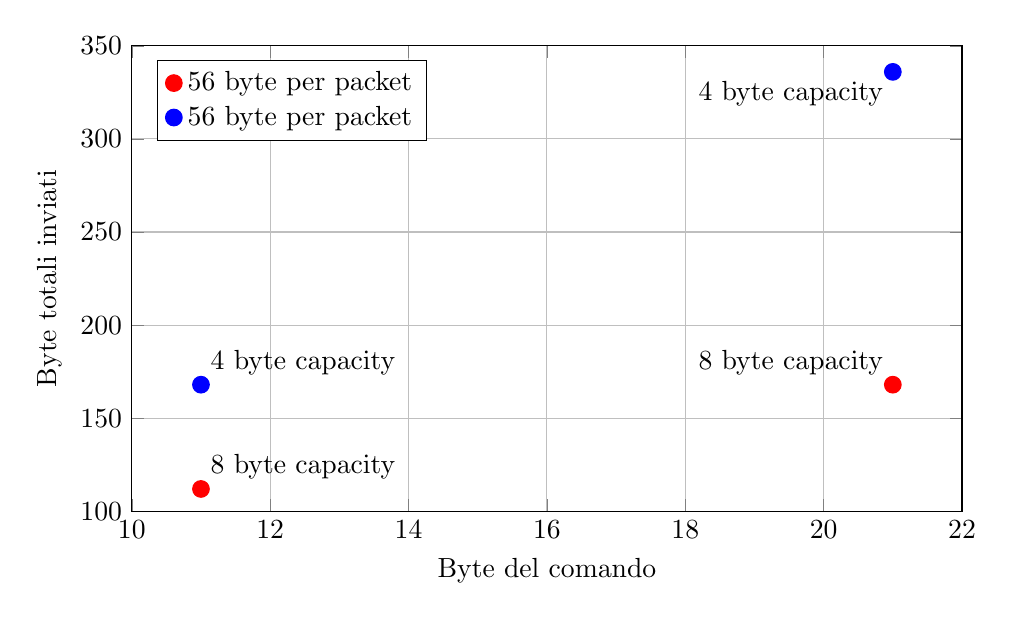
\begin{tikzpicture} 
    \tikzset{
    cmd11/.style={circle,fill=red,inner sep=2pt},
    cmd21/.style={circle,fill=blue,inner sep=2pt}
}
\begin{axis}[
    xlabel={Byte del comando}, 
    ylabel={Byte totali inviati},
    grid=major,
    width=\textwidth,
    height=0.618\textwidth, 
    domain=10:22,
    ymin=100,
    ymax=350, 
    legend pos=north west,
    legend entries={56 byte per packet, 56 byte per packet}
]  
% Plot points
\addplot[only marks, mark=*, mark size=3pt, red] 
coordinates {(11,112) (21,168)};
\addplot[only marks, mark=*, mark size=3pt, blue] 
coordinates {(11,168) (21,336)}; 
%\addplot[only marks, mark=*, mark size=3pt, Cerulean] 
%coordinates {(11,108) (21,216)}; 
%\addplot[only marks, mark=*, mark size=3pt, orange] 
%coordinates {(11,58) (21,87)}; 
% Add labels for the points 
\node[above right] at (axis cs:11,112) {8 byte capacity};
\node[above left] at (axis cs:21,168) {8 byte capacity};
\node[above right] at (axis cs:11,168) {4 byte capacity}; 
\node[below left] at (axis cs:21,336) {4 byte capacity}; 

%\node[right] at (axis cs:11,108) {2nd version};
%\node[left] at (axis cs:21,216) {2nd version};
%\node[right] at (axis cs:11,58) {2nd version}; 
%\node[left] at (axis cs:21,87) {2nd version}; 

\end{axis}
\end{tikzpicture}
\caption{Analisi tempi esecuzione \textit{Destination Unreachable}} 
\label{table:destunreach6:bytetotali:bytecomando}
\end{center}
Dall'analisi segue che il metodo \hyperref[destunreach6:casoA]{A} risulti il migliore. 
Infatti potrebbe essere facilmente rilevato semplicemente analizzando il campo \textit{unused} ma spedisce meno pacchetti per inviare il comando. 
Ciò risulta in un minor numero di bytes spediti in totale. 
\vspace{1ex} \newline 
Invece il secondo, per quanto corretto nelle norme, invia un numero considerevole di pacchetti (e quindi di bytes) rispetto alla controparte. 
Questo può rappresentare un problema maggiore siccome lo rende maggiormente rilevabile. 
Infatti un metodo di difesa potrebbe non accorgersi del campo \textit{unused} ma con molta probabilità si renderà conto della quantità di bytes ricevuti. 
\vspace{2ex} \newline
Un'\textbf{alternativa} potrebbe essere quella di \textbf{usare il campo} \textit{unused} e 
\textbf{strutturare il pacchetto} usando nel datagram aggiuntivo diversi protocolli o tipologie di messaggi ICMP 
che permettano l'inserimento di un maggior numero di bytes e al tempo stesso che riduca il numero di bytes per pacchetto. 
\vspace{1ex} \newline 
Nel nostro caso il datagram aggiuntivo usa la tipologia \textit{ICMP Echo Request}. 
Anche se potrebbe essere sostituito da una tipologia avente il campo \textit{unused} o \textit{mtu} (e.g \textit{Time Exceeded}, \textit{Packet Too Big}). 
Ma in questo caso la cosa potrebbe risultare meno probabile rispetto alla tipologia \textit{Echo Request}. 
Infatti si potrebbe supporre che l'utente abbia fatto ping ma che la connesisone non sia presente. 
\vspace{2ex} \newline
Di conseguenza questa alternativa non verrà fatta e si procederà usando la struttra \hyperref[destunreach6:casoA]{A}. 


\subsubsection{Packet Too Big Message (ICMPv6)} 
Nel protocollo \textbf{ICMPv6} la tipologia di messaggio \textit{Packet Too Big}, 
viene generato da un router in risposta a un pacchetto che non può inoltrare perché esso è più grande dell'MTU del collegamento in uscita.
Le informazioni contenute in questo messaggio vengono utilizzate come parte del processo di \href{https://www.rfc-editor.org/rfc/rfc4443#ref-PMTU}{Path MTU Discovery}.
%Originating a Packet Too Big Message makes an exception to one of the rules as to when to originate an ICMPv6 error message.  
%Unlike other messages, it is sent in response to a packet received with an IPv6 multicast destination address, or with a link-layer multicast or link-layer broadcast address. 
Un nodo che riceve un messaggio ICMPv6 \textit{Packet Too Big} deve notificare la cosa al 
processo di livello superiore (se il processo in questione può essere identificato). 

\subsubsection*{Struttura del pacchetto} 
\begin{bytefield}[bitwidth=1.1em]{32} 
    %\bitbox{8}{0} & \bitbox{8}{1} & \bitbox{8}{2} & \bitbox{8}{3} \\
    \bitheader{0-31} \\
    \bitbox{8} {Type (1B)} & \bitbox{8}{Code (1B)} & \bitbox{16}{Checksum (2B)} \\
    \bitbox{32} {MTU (4B)} \\
    \bitbox{32} {As much of invoking packet as possible without} \\
    \bitbox{32} {the ICMPv6 packet exceeding the minimum IPv6 MTU ($\geq$ 0B)} 
\end{bytefield}
I campi sono i seguenti: 
\begin{itemize}
    \item Type: 2 
    \item Code: 0 impostato dal mittente ed ignorato dal destinatario
    \item Checksum: è il complemento a 16 bit del complemento a uno relativo alla somma del messaggio ICMP 
    (che inizia con il campo Type). Verrà calcolato se il campo è zero. 
    \item MTU: la massima unità di trasmissione del collegamento del salto successivo 
    \item Invoking Packet: quanta parte del pacchetto (che ha attivato l'errore ICMPv6) debba essere inclusa. 
    Il tutto senza eccedere il \textit{IPv6 MTU} che equivale a \href{https://www.rfc-editor.org/rfc/rfc2460#section-5}{\textbf{1280 bytes}}. 
    \footnote{\textbf{MTU}=maximum transmission unit ovvero il massimo carico possibile} 
    \footnote{L'\textit{intestazione IP} contiene al minimo 40 byte} 
\end{itemize} 
\vspace{1ex} 
Si sfrutteranno quindi i campi nel seguente modo: 
\begin{itemize}
    \item Il campo \textbf{checksum} non è utilizzabile. 
    Essendo il complemento ad 1 del contenuto del pacchetto, se non combaciasse il pacchetto verrebbe scartato. 
    \item Il campo \textbf{mtu} può contenere i dati e, siccome rappresenta la cpacità del collegamento, potrà essere variabile. 
    E quindi potremmo inserire al suo interno \textit{4 bytes}. 
    \item Nel campo \textbf{Invoking Packet} si userà il campo \textbf{plen} del protocollo \textit{IPv6} e il campo \textbf{id} del protocollo \textit{ICMPv6}. 
    Tuttavia, in questo caso si dovrà stare attenti a non superare la \textit{IPv6 MTU}, 
    ma ciò non succederà siccome l'intestazione IPv6 sarà di 40 byte emntre l'intestazione ICMPv6 sarà di 8 byte. 
\end{itemize} 

\subsubsection*{Analisi complessiva} 
Per l'analisi supponiamo di mandare due comandi che sono: 
\begin{itemize}
    \item \textbf{echo 'Ciao'}: che sono \textit{11 byte} (e quindi \textit{88 bit}\footnote{\label{note:pktbig6:analisi}Ciò sarà utile per i \textit{Timing Covert Channel}})
    \item \textbf{cd /home/marco; ls -l}: che sono \textit{21 byte}  (e quindi \textit{168 bit}\textsuperscript{\ref{note:pktbig6:analisi}}) %\footnotemark[2]
\end{itemize}
Sappiamo che nel caso migliore la capacità di trasmissione di ogni pacchetto è \textbf{8 byte} \label{pktbig6:casoA}. 
Siccome si userà il campo \textit{mtu} mentre nel datagram aggiuntivo il campo \textit{pleng} e il campo \textit{id} (del protocollo ICMPv6 Echo)
\vspace{1ex} \newline
Per ogni comando si confronteranno entrambe le varianti considerando che: 
\begin{itemize}
    \item Ogni pacchetto del primo caso (che chiameremo \hyperref[pktbig6:casoA]{A}) trasporterà \textbf{56 byte} 
    \footnote{8 per i campi ICMP + 40 del datagram IP + 8 del datagram ICMP} 
\end{itemize} 
Ora procediamo ad analizzare quanti pacchetti sono necessari per inviare i comandi. \newline
Nel caso si mandasse il comando \textbf{echo 'Ciao'} il numero di pacchetti necessari sarebbere: 
\begin{itemize}
    \item Caso \hyperref[pktbig6:casoA]{A}: Sarebbero necessari \textit{due pacchetti}. 
    E quindi siccome ogni pacchetto trasporta 56 byte; si spediranno in totale \textbf{112 byte}. 
\end{itemize} 
Ora analiziamo il comando \textbf{cd /home/marco; ls -l} e quanti pacchetti saranno necessari: 
\begin{itemize}
    \item Caso \hyperref[pktbig6:casoA]{A}: siccome è di \textit{21 byte}, servirebbero \textit{3 pacchetti}. 
    Quindi siccome ogni pacchetto trasporta 56 byte; si spediranno in totale \textbf{168 byte}. 
\end{itemize}

\begin{center} 
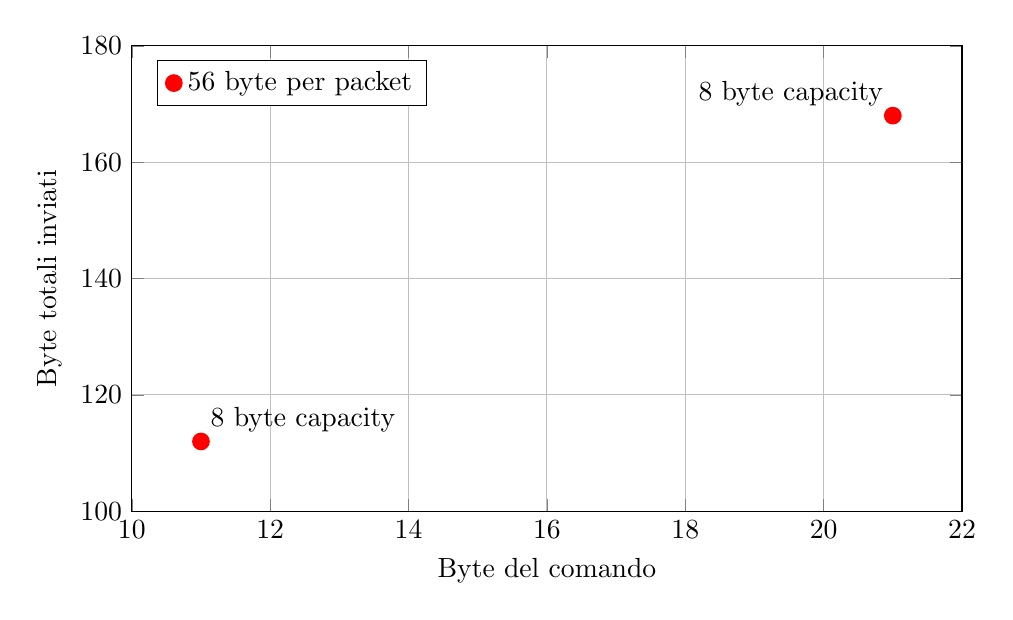
\begin{tikzpicture} 
    \tikzset{
    cmd11/.style={circle,fill=red,inner sep=2pt},
    cmd21/.style={circle,fill=blue,inner sep=2pt}
}
\begin{axis}[
    xlabel={Byte del comando}, 
    ylabel={Byte totali inviati},
    grid=major,
    width=\textwidth,
    height=0.618\textwidth, 
    domain=10:22,
    ymin=100,
    ymax=180, 
    legend pos=north west,
    legend entries={56 byte per packet, 56 byte per packet}
]  
% Plot points
\addplot[only marks, mark=*, mark size=3pt, red] 
coordinates {(11,112) (21,168)}; 
%\addplot[only marks, mark=*, mark size=3pt, Cerulean] 
%coordinates {(11,108) (21,216)}; 
%\addplot[only marks, mark=*, mark size=3pt, orange] 
%coordinates {(11,58) (21,87)}; 
% Add labels for the points 
\node[above right] at (axis cs:11,112) {8 byte capacity};
\node[above left] at (axis cs:21,168) {8 byte capacity};
%\node[above right] at (axis cs:11,168) {4 byte capacity}; 
%\node[below left] at (axis cs:21,336) {4 byte capacity}; 

%\node[right] at (axis cs:11,108) {2nd version};
%\node[left] at (axis cs:21,216) {2nd version};
%\node[right] at (axis cs:11,58) {2nd version}; 
%\node[left] at (axis cs:21,87) {2nd version}; 

\end{axis}
\end{tikzpicture}
\caption{Analisi tempi esecuzione \textit{Packet too Big}} 
\label{table:pktbig6:bytetotali:bytecomando}
\end{center}
L'unico metodo presente è \hyperref[pktbig6:casoA]{A}; quindi risulterà il migliore ma perchè non ci sono confronti. 
\vspace{2ex} \newline
Un'\textbf{alternativa} potrebbe essere quella di \textbf{strutturare il pacchetto} usando nel datagram aggiuntivo diversi protocolli o 
tipologie di messaggi ICMP che permettano l'inserimento di un maggior numero di bytes e al tempo stesso che riduca il numero di bytes per pacchetto. 
\vspace{1ex} \newline 
Nel nostro caso il datagram aggiuntivo usa la tipologia \textit{ICMP Echo Request}. 
Anche se potrebbe essere sostituito da una tipologia avente il campo \textit{unused} o \textit{mtu} (e.g \textit{Time Exceeded}, \textit{Packet Too Big}). 
Ma in questo caso la cosa potrebbe risultare meno probabile rispetto alla tipologia \textit{Echo Request}. 
Infatti si potrebbe supporre che l'utente abbia fatto ping ma che la connesisone non sia presente. 
\vspace{2ex} \newline 
Di conseguenza questa alternativa non verrà usata e si procederà usando la struttra \hyperref[pktbig6:casoA]{A}. 


\subsubsection{Time Exceeded Message (ICMPv6)} 
Nel protocollo \textbf{ICMPv6} la tipologia di messaggio \textit{Time Exceeded}, 
viene generato se un router riceve un pacchetto con un limite di hop pari a zero,  
o se un router decrementa il limite di hop di un pacchetto a zero. 
In questi casi si dovrà scartare il pacchetto e inviare al mittente un messaggio \textit{Time Exceeded} con codice 0. 
Ciò indica un loop nel routing o un valore iniziale della quantità di hop possibili troppo basso.
Un messaggio \textit{Time Exceeded} con codice 1 invece viene utilizzato per segnalare il timeout nel riassemblaggio dei frammenti. 
\vspace{1ex} \newline 
I codici associati ai possibili casi sono i seguenti: 
\begin{itemize}
    \item[0] Limite degli hop superato durante il transito 
    \item[1] Tempo per riassemblare i frammenti superato
\end{itemize}
Un nodo che riceve un messaggio ICMPv6 \textit{Time Exceeded} deve notificare la cosa al 
processo di livello superiore (se il processo in questione può essere identificato).

\subsubsection*{Struttura del pacchetto} 
\begin{bytefield}[bitwidth=1.1em]{32} 
    %\bitbox{8}{0} & \bitbox{8}{1} & \bitbox{8}{2} & \bitbox{8}{3} \\
    \bitheader{0-31} \\
    \bitbox{8} {Type (1B)} & \bitbox{8}{Code (1B)} & \bitbox{16}{Checksum (2B)} \\
    \bitbox{32} {Unused (4B)} \\
    \bitbox{32} {As much of invoking packet as possible without} \\
    \bitbox{32} {the ICMPv6 packet exceeding the minimum IPv6 MTU ($\geq$ 0B)} 
\end{bytefield}
I campi sono i seguenti: 
\begin{itemize}
    \item Type: 3 
    \item Code: 0-1 
    \item Checksum: è il complemento a 16 bit del complemento a uno relativo alla somma del messaggio ICMP 
    (che inizia con il campo Type). Verrà calcolato se il campo è zero. 
    \item Unused: il campo non è utilizzato per tutti i codici possibili.
    Deve essere inizializzato a zero dal mittente e ignorato dal destinatario. 
    \item Invoking Packet: quanta parte del pacchetto (che ha attivato l'errore ICMPv6) debba essere inclusa. 
    Il tutto senza eccedere il \textit{IPv6 MTU} che equivale a \href{https://www.rfc-editor.org/rfc/rfc2460#section-5}{\textbf{1280 bytes}}. 
    \footnote{\textbf{MTU}=maximum transmission unit ovvero il massimo carico possibile} 
    \footnote{L'\textit{intestazione IP} contiene al minimo 40 byte} 
\end{itemize} 
\vspace{1ex} 
Si sfrutteranno quindi i campi nel seguente modo: 
\begin{itemize}
    \item Il campo \textbf{checksum} non è utilizzabile. 
    Essendo il complemento ad 1 del contenuto del pacchetto, se non combaciasse il pacchetto verrebbe scartato. 
    \item Il campo \textbf{unused} dalle specifiche \href{https://www.rfc-editor.org/rfc/rfc4443#section-3.3}{RFC 4434} dovrebbe essere 0. 
    Tuttavia nel nostro caso è stato utilizzato per testare la presenza della \textit{Deep Packet Inspection}. 
    \item Nel campo \textbf{Invoking Packet} si userà il campo \textbf{plen} del protocollo \textit{IPv6} e il campo \textbf{id} del protocollo \textit{ICMPv6}. 
    Tuttavia, in questo caso si dovrà stare attenti a non superare la \textit{IPv6 MTU}, 
    ma ciò non succederà siccome l'intestazione IPv6 sarà di 40 byte emntre l'intestazione ICMPv6 sarà di 8 byte. 
\end{itemize} 

\subsubsection*{Analisi complessiva} 
Per l'analisi supponiamo di mandare due comandi che sono: 
\begin{itemize}
    \item \textbf{echo 'Ciao'}: che sono \textit{11 byte} (e quindi \textit{88 bit}\footnote{\label{note:timexceed6:analisi}Ciò sarà utile per i \textit{Timing Covert Channel}})
    \item \textbf{cd /home/marco; ls -l}: che sono \textit{21 byte}  (e quindi \textit{168 bit}\textsuperscript{\ref{note:timexceed6:analisi}}) %\footnotemark[2]
\end{itemize}
Sappiamo che nel caso migliore la capacità di trasmissione di ogni pacchetto è \textbf{8 byte} \label{timexceed6:casoA}; 
mentre nel caso si vogliano rispettare le linee guida \href{https://www.rfc-editor.org/rfc/rfc4443#section-3.3}{RFC 4443}
non si potrà usare il campo \textit{unused}.
In questo secondo caso la capacità diventerà di \textbf{4 byte} \label{timexceed6:casoB} siccome il campo \textit{plen} e \textit{id} verranno utilizzati. 
\vspace{1ex} \newline
Per ogni comando si confronteranno entrambe le varianti considerando che: 
\begin{itemize}
    \item Ogni pacchetto del primo caso (che chiameremo \hyperref[timexceed6:casoA]{A}) trasporterà \textbf{56 byte} 
    \footnote{8 per i campi ICMP + 40 del datagram IP + 8 del datagram ICMP}
    \item Ogni pacchetto del secondo caso (che chiameremo \hyperref[timexceed6:casoB]{B}) trasporterà \textbf{56 byte}
    \footnote{8 per i campi ICMP + 40 del datagram IP + 1 byte del datagram}
\end{itemize} 
Ora procediamo ad analizzare quanti pacchetti sono necessari per inviare i comandi. \newline
Nel caso si mandasse il comando \textbf{echo 'Ciao'} il numero di pacchetti necessari sarebbere: 
\begin{itemize}
    \item Caso \hyperref[timexceed6:casoA]{A}: Sarebbero necessari \textit{due pacchetti}. 
    E quindi siccome ogni pacchetto trasporta 56 byte; si spediranno in totale \textbf{112 byte}.  
    \item Caso \hyperref[timexceed6:casoB]{B}: Sarebbero necessari \textit{4 pacchetti}. 
     E quindi siccome ogni pacchetto trasporta 56 byte; si spediranno in totale \textbf{168 byte}. 
\end{itemize} 
Ora analiziamo il comando \textbf{cd /home/marco; ls -l} e quanti pacchetti saranno necessari: 
\begin{itemize}
    \item Caso \hyperref[timexceed6:casoA]{A}: siccome è di \textit{21 byte}, servirebbero \textit{3 pacchetti}. 
    Quindi siccome ogni pacchetto trasporta 56 byte; si spediranno in totale \textbf{168 byte}.  
    \item Caso \hyperref[timexceed6:casoB]{B}: siccome è di \textit{21 byte}, servirebbero \textit{6 pacchetti}. 
    Quindi siccome ogni pacchetto trasporta 56 byte; si spediranno in totale \textbf{336 byte}.  
\end{itemize}

\begin{center} 
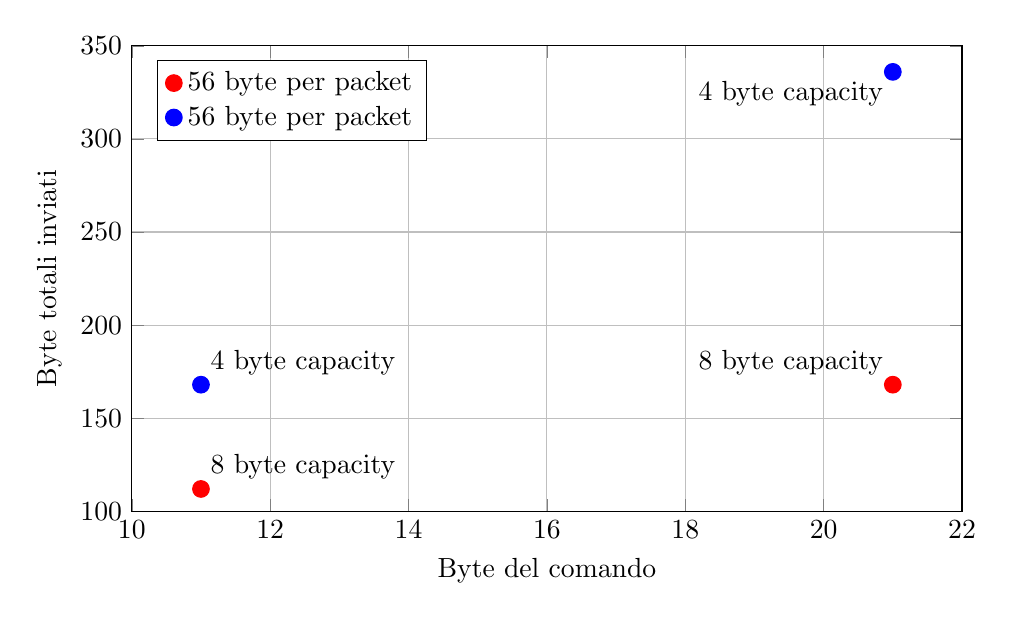
\begin{tikzpicture} 
    \tikzset{
    cmd11/.style={circle,fill=red,inner sep=2pt},
    cmd21/.style={circle,fill=blue,inner sep=2pt}
}
\begin{axis}[
    xlabel={Byte del comando}, 
    ylabel={Byte totali inviati},
    grid=major,
    width=\textwidth,
    height=0.618\textwidth, 
    domain=10:22,
    ymin=100,
    ymax=350, 
    legend pos=north west,
    legend entries={56 byte per packet, 56 byte per packet}
]  
% Plot points
\addplot[only marks, mark=*, mark size=3pt, red] 
coordinates {(11,112) (21,168)};
\addplot[only marks, mark=*, mark size=3pt, blue] 
coordinates {(11,168) (21,336)}; 

% Add labels for the points 
\node[above right] at (axis cs:11,112) {8 byte capacity};
\node[above left] at (axis cs:21,168) {8 byte capacity};
\node[above right] at (axis cs:11,168) {4 byte capacity}; 
\node[below left] at (axis cs:21,336) {4 byte capacity};  

\end{axis}
\end{tikzpicture}
\caption{Analisi tempi esecuzione \textit{Time Excedeed}} 
\label{table:timexceed6:bytetotali:bytecomando}
\end{center}
Dall'analisi segue che il metodo \hyperref[timexceed6:casoA]{A} risulti il migliore. 
Infatti potrebbe essere facilmente rilevato semplicemente analizzando il campo \textit{unused} ma spedisce meno pacchetti per inviare il comando. 
Ciò risulta in un minor numero di bytes spediti in totale. 
\vspace{1ex} \newline 
Invece il secondo, per quanto corretto nelle norme, invia un numero considerevole di pacchetti (e quindi di bytes) rispetto alla controparte. 
Questo può rappresentare un problema maggiore siccome lo rende maggiormente rilevabile. 
Infatti un metodo di difesa potrebbe non accorgersi del campo \textit{unused} ma con molta probabilità si renderà conto della quantità di bytes ricevuti. 
\vspace{2ex} \newline
Un'\textbf{alternativa} potrebbe essere quella di \textbf{usare il campo} \textit{unused} e 
\textbf{strutturare il pacchetto} usando nel datagram aggiuntivo diversi protocolli o tipologie di messaggi ICMP 
che permettano l'inserimento di un maggior numero di bytes e al tempo stesso che riduca il numero di bytes per pacchetto. 
\vspace{1ex} \newline 
Nel nostro caso il datagram aggiuntivo usa la tipologia \textit{ICMP Echo Request}. 
Anche se potrebbe essere sostituito da una tipologia avente il campo \textit{unused} o \textit{mtu} (e.g \textit{Time Exceeded}, \textit{Packet Too Big}). 
Ma in questo caso la cosa potrebbe risultare meno probabile rispetto alla tipologia \textit{Echo Request}. 
Infatti si potrebbe supporre che l'utente abbia fatto ping ma che la connesisone non sia presente. 
\vspace{2ex} \newline
Di conseguenza questa alternativa non verrà fatta e si procederà usando la struttra \hyperref[timexceed6:casoA]{A}. 


\subsubsection{Parameter Problem Message (ICMPv6)} 
Nel protocollo \textbf{ICMPv6} la tipologia di messaggio \textit{Parameter Problem}, 
viene generato se un nodo che elabora un pacchetto, rileva un problema con un campo nell'intestazione IPv6 o 
nelle intestazioni di estensione tale da impedirgli di completare l'elaborazione di esso. 
Di conseguenza deve scartare il pacchetto e inviare un messaggio ICMPv6 Parameter Problem alla sorgente del pacchetto, indicando il tipo e la posizione del problema. 
\vspace{1ex} \newline 
I codici associati ai possibili casi sono i seguenti: 
\begin{itemize} 
    \item[0] Campo di intestazione errato  
    \item[1] Tipologia del Next Header non riconosciuta 
    \item[2] Opzione IPv6 non riconosciuta 
\end{itemize} 
Un nodo che riceve un messaggio ICMPv6 \textit{Parameter Problem} deve notificare la cosa al processo di livello superiore (se il processo in questione può essere identificato).

\subsubsection*{Struttura del pacchetto} 
\begin{bytefield}[bitwidth=1.1em]{32} 
    \bitheader{0-31} \\
    \bitbox{8} {Type (1B)} & \bitbox{8}{Code (1B)} & \bitbox{16}{Checksum (2B)} \\
    \bitbox{32} {Pointer (4B)} \\
    \bitbox{32} {As much of invoking packet as possible without} \\
    \bitbox{32} {the ICMPv6 packet exceeding the minimum IPv6 MTU ($\geq$ 0B)} 
\end{bytefield}
I campi sono i seguenti: 
\begin{itemize}
    \item Type: 4 
    \item Code: 0-2
    \item Checksum: è il complemento a 16 bit del complemento a uno relativo alla somma del messaggio ICMP 
    (che inizia con il campo Type). Verrà calcolato se il campo è zero. 
    \item Pointer: identifica l'ottetto nell'intestazione del pacchetto originale in cui è stato rilevato l'errore
    \item Invoking Packet: quanta parte del pacchetto (che ha attivato l'errore ICMPv6) debba essere inclusa. 
    Il tutto senza eccedere il \textit{IPv6 MTU} che equivale a \href{https://www.rfc-editor.org/rfc/rfc2460#section-5}{\textbf{1280 bytes}}. 
    \footnote{\textbf{MTU}=maximum transmission unit ovvero il massimo carico possibile} 
    \footnote{L'\textit{intestazione IP} contiene al minimo 40 byte} 
\end{itemize} 
\vspace{1ex} 
Si sfrutteranno quindi i campi nel seguente modo: 
\begin{itemize}
    \item Il campo \textbf{checksum} non è utilizzabile. 
    Essendo il complemento ad 1 del contenuto del pacchetto, se non combaciasse il pacchetto verrebbe scartato. 
    \item Il campo \textbf{pointer} può contenere i dati e, siccome rappresenta l'ottetto in cui è stato rilevato l'errore, potrà essere variabile. 
    E quindi potremmo inserire al suo interno \textit{4 bytes}. 
    \item Nel campo \textbf{Invoking Packet} si userà il campo \textbf{plen} del protocollo \textit{IPv6} e il campo \textbf{id} del protocollo \textit{ICMPv6}. 
    Tuttavia, in questo caso si dovrà stare attenti a non superare la \textit{IPv6 MTU}, 
    ma ciò non succederà siccome l'intestazione IPv6 sarà di 40 byte emntre l'intestazione ICMPv6 sarà di 8 byte. 
\end{itemize} 

\subsubsection*{Analisi complessiva} 
Per l'analisi supponiamo di mandare due comandi che sono: 
\begin{itemize}
    \item \textbf{echo 'Ciao'}: che sono \textit{11 byte} (e quindi \textit{88 bit}\footnote{\label{note:paramproblem6:analisi}Ciò sarà utile per i \textit{Timing Covert Channel}})
    \item \textbf{cd /home/marco; ls -l}: che sono \textit{21 byte}  (e quindi \textit{168 bit}\textsuperscript{\ref{note:paramproblem6:analisi}}) %\footnotemark[2]
\end{itemize}
Sappiamo che nel caso migliore la capacità di trasmissione di ogni pacchetto è \textbf{8 byte} \label{paramproblem6:casoA}. 
Siccome si userà il campo \textit{pointer} mentre nel datagram aggiuntivo il campo \textit{pleng} e il campo \textit{id} (del protocollo ICMPv6 Echo)
\vspace{1ex} \newline
Per ogni comando si confronteranno entrambe le varianti considerando che: 
\begin{itemize}
    \item Ogni pacchetto del primo caso (che chiameremo \hyperref[paramproblem6:casoA]{A}) trasporterà \textbf{56 byte} 
    \footnote{8 per i campi ICMP + 40 del datagram IP + 8 del datagram ICMP} 
\end{itemize} 
Ora procediamo ad analizzare quanti pacchetti sono necessari per inviare i comandi. \newline
Nel caso si mandasse il comando \textbf{echo 'Ciao'} il numero di pacchetti necessari sarebbere: 
\begin{itemize}
    \item Caso \hyperref[paramproblem6:casoA]{A}: Sarebbero necessari \textit{due pacchetti}. 
    E quindi siccome ogni pacchetto trasporta 56 byte; si spediranno in totale \textbf{112 byte}. 
\end{itemize} 
Ora analiziamo il comando \textbf{cd /home/marco; ls -l} e quanti pacchetti saranno necessari: 
\begin{itemize}
    \item Caso \hyperref[paramproblem6:casoA]{A}: siccome è di \textit{21 byte}, servirebbero \textit{3 pacchetti}. 
    Quindi siccome ogni pacchetto trasporta 56 byte; si spediranno in totale \textbf{168 byte}. 
\end{itemize}

\begin{center} 
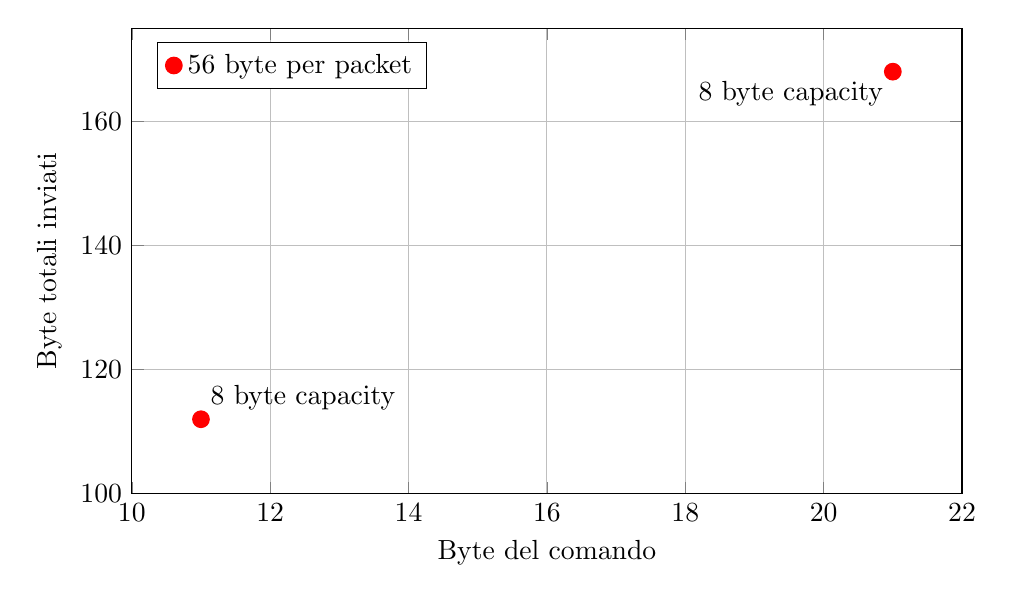
\begin{tikzpicture} 
    \tikzset{
    cmd11/.style={circle,fill=red,inner sep=2pt},
    cmd21/.style={circle,fill=blue,inner sep=2pt}
}
\begin{axis}[
    xlabel={Byte del comando}, 
    ylabel={Byte totali inviati},
    grid=major,
    width=\textwidth,
    height=0.618\textwidth, 
    domain=10:22,
    ymin=100,
    ymax=175, 
    legend pos=north west,
    legend entries={56 byte per packet, 56 byte per packet}
]  
% Plot points
\addplot[only marks, mark=*, mark size=3pt, red] 
coordinates {(11,112) (21,168)}; 
% Add labels for the points 
\node[above right] at (axis cs:11,112) {8 byte capacity};
\node[below left] at (axis cs:21,168) {8 byte capacity}; 

\end{axis}
\end{tikzpicture}
\caption{Analisi tempi esecuzione \textit{Parameter Problem}} 
\label{table:paramproblem6:bytetotali:bytecomando}
\end{center}
L'unico metodo presente è \hyperref[paramproblem6:casoA]{A}; quindi risulterà il migliore ma perchè non ci sono confronti. 
\vspace{2ex} \newline
Un'\textbf{alternativa} potrebbe essere quella di \textbf{strutturare il pacchetto} usando nel datagram aggiuntivo diversi protocolli o 
tipologie di messaggi ICMP che permettano l'inserimento di un maggior numero di bytes e al tempo stesso che riduca il numero di bytes per pacchetto. 
\vspace{1ex} \newline 
Nel nostro caso il datagram aggiuntivo usa la tipologia \textit{ICMP Echo Request}. 
Anche se potrebbe essere sostituito da una tipologia avente il campo \textit{unused} o \textit{mtu} (e.g \textit{Time Exceeded}, \textit{Packet Too Big}). 
Ma in questo caso la cosa potrebbe risultare meno probabile rispetto alla tipologia \textit{Echo Request}. 
Infatti si potrebbe supporre che l'utente abbia fatto ping ma che la connesisone non sia presente. 
\vspace{2ex} \newline 
Di conseguenza questa alternativa non verrà usata e si procederà usando la struttra \hyperref[paramproblem6:casoA]{A}. 


\subsubsection{Echo Request or Echo Reply Message (ICMPv6)} 
Nel protocollo \textbf{ICMPv6} la tipologia di messaggio \textit{Echo}, viene usata per ricevere indietro una risposta da un host. 
In questi casi, una \textit{Echo Reply} dovrebbe essere inviata in risposta alla messaggio di \textit{Echo Request}. 
E non vi è alcuna limitazione alla quantità di dati inseribili nei messaggi \textit{Echo}. 
\vspace{1ex} \newline 
I dati ricevuti dall \textit{Echo Request}, dovranno essere restituiti nel messaggio di risposta integralmente e senza modifiche. 
Inoltre i'identificatore e il numero di sequenza possono essere utilizzati dal 
mittente per facilitare l'abbinamento delle risposte con le richieste.
%Ad esempio, l'identificatore potrebbe essere utilizzato come una porta in TCP o UDP per identificare una 
%sessione e il numero di sequenza potrebbe essere incrementato a ogni richiesta di eco inviata.
Inoltre nel messaggio di \textit{Echo Reply}, l'indirizzo sorgente deve essere lo stesso dell'indirizzo di destinazione presente nel messaggio di \textit{Echo Request}.
\vspace{1ex} \newline 
Per creare un messaggio di risposta, gli indirizzi di origine e di destinazione vengono semplicemente invertiti,
il codice da 128 viene modificato in 129 e il checksum viene ricalcolato. 
In aggiunta, ogni nodo deve implementare una funzione di risposta ai messaggi \textit{Echo ICMPv6} così che 
quando riceve delle richieste Echo, generi le relative risposte. 
\vspace{2ex} \newline
%A node SHOULD also implement an application-layer interface for originating Echo Requests and receiving Echo Replies, for diagnostic purposes.
%E inoltre, un nodo dovrebbe implementare un'interfaccia a livello applicazione per poter generare Richieste Echo e ricevere Risposte Echo, a fini diagnostici.
I messaggi \textit{Echo Request} possono essere passati ai processi che ricevono i messaggi \textit{ICMP}. 
Identica cosa i messaggi di \textit{Echo Reply}. 
Essi devono essere trasmessi al processo che ha originato il messaggio di richiesta. 
Inoltre un messaggio di risposta, può essere trasmesso a processi che non hanno originato il messaggio \textit{Echo Request}. 

\subsubsection*{Struttura del pacchetto} 
\begin{bytefield}[bitwidth=1.1em]{32} 
    %\bitbox{8}{0} & \bitbox{8}{1} & \bitbox{8}{2} & \bitbox{8}{3} \\
    \bitheader{0-31} \\
    \bitbox{8}{Type (1B)} & \bitbox{8}{Code (1B)} & \bitbox{16}{Checksum (2B)} \\
    \bitbox{16}{Identifier (2B)} && \bitbox{16}{Sequence Number (2B)} \\
    \bitbox{32}{Data ... ($\geq$ 0B)} 
\end{bytefield}
I campi sono i seguenti: 
\begin{itemize} 
    \item Type: 128 per i messaggi Echo Request; 129 per i messaggi Echo Reply.
    \item Code: 0 
    \item Checksum: è il complemento a 16 bit del complemento a uno relativo alla somma del messaggio ICMP 
    (che inizia con il campo Type). Verrà calcolato se il campo è zero. 
    \item Identifier: se il codice = 0; l'identificatore serve per facilitare la corrispondenza tra le richieste Echo e le Risposte Echo. Può essere zero. 
    \item Sequence Number: se il codice = 0; il numero di sequenza serve per facilitare la corrispondenza tra le richieste Echo e le Risposte Echo. Può essere zero. 
\end{itemize}
\vspace{1ex} 
Si sfrutteranno quindi i campi nel seguente modo: 
\begin{itemize}
    \item Il campo \textbf{checksum} non è utilizzabile. 
    Essendo il complemento ad 1 del contenuto del pacchetto, se non combaciasse il pacchetto verrebbe scartato. 
    \item Il campo \textbf{identifier} che siccome serve a definire un identificativo delle richieste, può essere un qualsiasi valore. 
    \item Il campo di \textbf{sequenza} potrebbe essere utilizzato per inserire le informazioni; 
    tuttavia, dalle specifiche \href{https://www.rfc-editor.org/rfc/rfc4443#section-4.1}{RFC 4443}, esso viene incrementato ad ogni richiesta inviata. 
    Quindi se il valore del campo è troppo variabile, potrebbe risultare sospetto. 
\end{itemize}

\subsubsection*{Analisi complessiva} 
Per l'analisi supponiamo di mandare due comandi che sono: 
\begin{itemize}
    \item \textbf{echo 'Ciao'}: che sono \textit{11 byte} (e quindi \textit{88 bit}\footnote{\label{note:echo6:analisi}Ciò sarà utile per i \textit{Timing Covert Channel}})
    \item \textbf{cd /home/marco; ls -l}: che sono \textit{21 byte}  (e quindi \textit{168 bit}\textsuperscript{\ref{note:echo6:analisi}}) %\footnotemark[2]
\end{itemize}
Sappiamo che nel caso migliore la capacità di trasmissione di ogni pacchetto è \textbf{2 byte} \label{echo6:casoA}; 
questo perchè il campo \textit{identifier} ha una lunghezza di soli \textit{2 byte}. %20
\begin{itemize}
    \item Ogni pacchetto del caso (che chiameremo \hyperref[echo6:casoA]{A}) trasporterà \textbf{8 byte}
    \footnote{8 per i campi ICMP}
    (supponendo che non si inseriscano dati) 
\end{itemize} 
Ora si analizza quanti pacchetti saranno necessari per inviare i comandi. \newline
Nel caso si mandasse il comando \textbf{echo 'Ciao'} il numero di pacchetti necessari sarebbere: 
\begin{itemize}
    \item Caso \hyperref[echo6:casoA]{A}: Sarebbero necessari \textit{6 pacchetti}. 
    E quindi siccome ogni pacchetto trasporta \textit{8 byte}; si spediranno in totale \textbf{48 byte}. 
\end{itemize} 
Ora analiziamo il comando \textbf{cd /home/marco; ls -l} e quanti pacchetti saranno necessari: 
\begin{itemize}
    \item Caso \hyperref[echo6:casoA]{A}: siccome è di \textit{21 byte}, servirebbero \textit{11 pacchetti}. 
    Quindi siccome ogni pacchetto trasporta \textit{8 byte}; si spediranno in totale \textbf{88 byte}. 
\end{itemize}

\begin{center} 
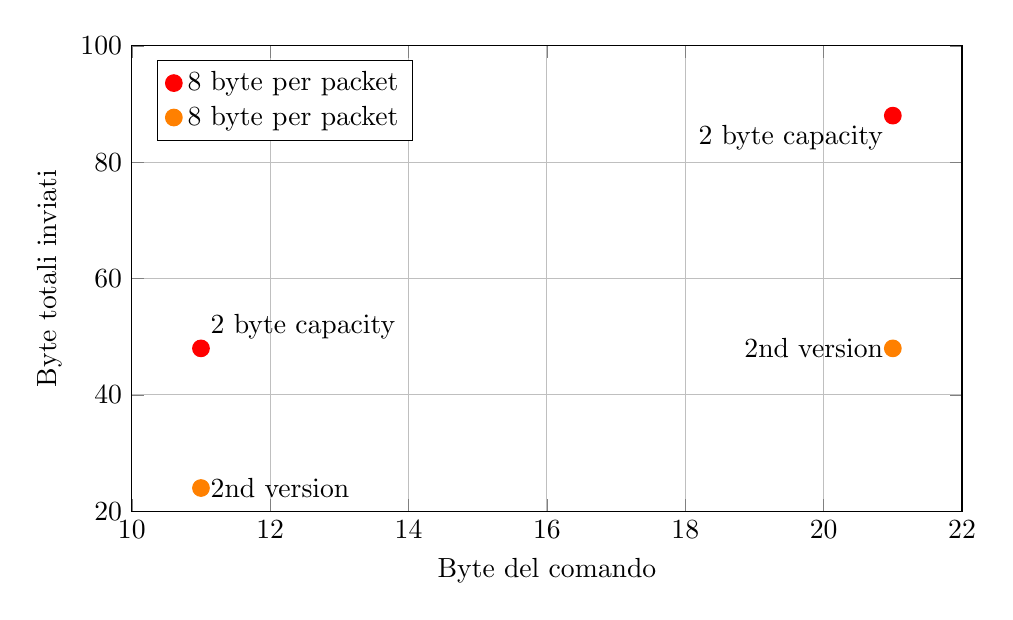
\begin{tikzpicture} 
    \tikzset{
    cmd11/.style={circle,fill=red,inner sep=2pt},
    cmd21/.style={circle,fill=blue,inner sep=2pt}
}
\begin{axis}[
    xlabel={Byte del comando}, 
    ylabel={Byte totali inviati},
    grid=major,
    width=\textwidth,
    height=0.618\textwidth, 
    domain=10:22,
    ymin=20,
    ymax=100, 
    legend pos=north west,
    legend entries={8 byte per packet, 8 byte per packet}
]  
% Plot points
\addplot[only marks, mark=*, mark size=3pt, red] 
coordinates {(11,48) (21,88)}; 
\addplot[only marks, mark=*, mark size=3pt, orange] 
coordinates {(11,24) (21,48)}; 
% Add labels for the points 
\node[above right] at (axis cs:11,48) {2 byte capacity}; 
\node[below left] at (axis cs:21,88) {2 byte capacity}; 

\node[right] at (axis cs:11,24) {2nd version}; 
\node[left] at (axis cs:21,48) {2nd version}; 

\end{axis}
\end{tikzpicture}
\caption{Analisi tempi esecuzione \textit{Echo}} 
\label{table:echo6:bytetotali:bytecomando}
\end{center}
Dall'analisi segue che il metodo \hyperref[echo6:casoA]{A} non riuslta il migliore. 
Infatti analizzando il caso in cui si usasse anche il campo di \textit{sequenza} [Tabella:\ref{table:echo6:bytetotali:bytecomando} Arancione]; 
si avrà una notevole differenza di bytes spediti totalmente rispetto al caso \hyperref[echo6:casoA]{A}. 
Tuttavia siccome l'uso di questo campo comporta una maggiore visibilità, 
si sceglie di non usarlo e correre il rischio. Questo comporterà l'invio di un maggior numero di bytes; 
che anche ciò potrebbe rivelare il Covert Channel. 
\vspace{1ex} \newline 
Si è scelto quindi di usare il metodo \hyperref[echo6:casoA]{A} ed affidarsi ai meccanismi di difesa presenti nella vittima; 
nella speranza che un numero elevato di pacchetti, ma senza il campo \textit{dati}, possano essere considerati innocqui.
\vspace{2ex} \newline 
Un \textbf{metodo maggiormente efficace} è proprio l'uso del campo \textbf{data}. 
Tuttavia anche questo approccio potrebbe destare sospetti. 
Infatti si dovrà decidere se mandare i dati in chiaro o cifrati:
\begin{itemize}
    \item Nel primo caso sarà possibile leggerne il contenuto. 
    \item Nell'altro, invece, la non possibilità di leggerne il ocntenuto rende lo scambio sospetto. 
    Siccome esistono canali migliori per poter scambiare informazioni in questo modo. 
\end{itemize} 
Inoltre bisognerebbe calcolare la capacità minima afifnche questo campo non risulti anomalo, ma sicuramente sarà maggiore di 2 byte. 
Questo lo si può affermare dopo aver testato i programmi di ping sia su Linux che su Windows. 

